
\documentclass{article} % For LaTeX2e
\usepackage{iclr2023_conference,times}

% Optional math commands from https://github.com/goodfeli/dlbook_notation.
%%%%% NEW MATH DEFINITIONS %%%%%

\usepackage{amsmath,amsfonts,bm}

% Mark sections of captions for referring to divisions of figures
\newcommand{\figleft}{{\em (Left)}}
\newcommand{\figcenter}{{\em (Center)}}
\newcommand{\figright}{{\em (Right)}}
\newcommand{\figtop}{{\em (Top)}}
\newcommand{\figbottom}{{\em (Bottom)}}
\newcommand{\captiona}{{\em (a)}}
\newcommand{\captionb}{{\em (b)}}
\newcommand{\captionc}{{\em (c)}}
\newcommand{\captiond}{{\em (d)}}

% Highlight a newly defined term
\newcommand{\newterm}[1]{{\bf #1}}


% Figure reference, lower-case.
\def\figref#1{figure~\ref{#1}}
% Figure reference, capital. For start of sentence
\def\Figref#1{Figure~\ref{#1}}
\def\twofigref#1#2{figures \ref{#1} and \ref{#2}}
\def\quadfigref#1#2#3#4{figures \ref{#1}, \ref{#2}, \ref{#3} and \ref{#4}}
% Section reference, lower-case.
\def\secref#1{section~\ref{#1}}
% Section reference, capital.
\def\Secref#1{Section~\ref{#1}}
% Reference to two sections.
\def\twosecrefs#1#2{sections \ref{#1} and \ref{#2}}
% Reference to three sections.
\def\secrefs#1#2#3{sections \ref{#1}, \ref{#2} and \ref{#3}}
% Reference to an equation, lower-case.
\def\eqref#1{equation~\ref{#1}}
% Reference to an equation, upper case
\def\Eqref#1{Equation~\ref{#1}}
% A raw reference to an equation---avoid using if possible
\def\plaineqref#1{\ref{#1}}
% Reference to a chapter, lower-case.
\def\chapref#1{chapter~\ref{#1}}
% Reference to an equation, upper case.
\def\Chapref#1{Chapter~\ref{#1}}
% Reference to a range of chapters
\def\rangechapref#1#2{chapters\ref{#1}--\ref{#2}}
% Reference to an algorithm, lower-case.
\def\algref#1{algorithm~\ref{#1}}
% Reference to an algorithm, upper case.
\def\Algref#1{Algorithm~\ref{#1}}
\def\twoalgref#1#2{algorithms \ref{#1} and \ref{#2}}
\def\Twoalgref#1#2{Algorithms \ref{#1} and \ref{#2}}
% Reference to a part, lower case
\def\partref#1{part~\ref{#1}}
% Reference to a part, upper case
\def\Partref#1{Part~\ref{#1}}
\def\twopartref#1#2{parts \ref{#1} and \ref{#2}}

\def\ceil#1{\lceil #1 \rceil}
\def\floor#1{\lfloor #1 \rfloor}
\def\1{\bm{1}}
\newcommand{\train}{\mathcal{D}}
\newcommand{\valid}{\mathcal{D_{\mathrm{valid}}}}
\newcommand{\test}{\mathcal{D_{\mathrm{test}}}}

\def\eps{{\epsilon}}


% Random variables
\def\reta{{\textnormal{$\eta$}}}
\def\ra{{\textnormal{a}}}
\def\rb{{\textnormal{b}}}
\def\rc{{\textnormal{c}}}
\def\rd{{\textnormal{d}}}
\def\re{{\textnormal{e}}}
\def\rf{{\textnormal{f}}}
\def\rg{{\textnormal{g}}}
\def\rh{{\textnormal{h}}}
\def\ri{{\textnormal{i}}}
\def\rj{{\textnormal{j}}}
\def\rk{{\textnormal{k}}}
\def\rl{{\textnormal{l}}}
% rm is already a command, just don't name any random variables m
\def\rn{{\textnormal{n}}}
\def\ro{{\textnormal{o}}}
\def\rp{{\textnormal{p}}}
\def\rq{{\textnormal{q}}}
\def\rr{{\textnormal{r}}}
\def\rs{{\textnormal{s}}}
\def\rt{{\textnormal{t}}}
\def\ru{{\textnormal{u}}}
\def\rv{{\textnormal{v}}}
\def\rw{{\textnormal{w}}}
\def\rx{{\textnormal{x}}}
\def\ry{{\textnormal{y}}}
\def\rz{{\textnormal{z}}}

% Random vectors
\def\rvepsilon{{\mathbf{\epsilon}}}
\def\rvtheta{{\mathbf{\theta}}}
\def\rva{{\mathbf{a}}}
\def\rvb{{\mathbf{b}}}
\def\rvc{{\mathbf{c}}}
\def\rvd{{\mathbf{d}}}
\def\rve{{\mathbf{e}}}
\def\rvf{{\mathbf{f}}}
\def\rvg{{\mathbf{g}}}
\def\rvh{{\mathbf{h}}}
\def\rvu{{\mathbf{i}}}
\def\rvj{{\mathbf{j}}}
\def\rvk{{\mathbf{k}}}
\def\rvl{{\mathbf{l}}}
\def\rvm{{\mathbf{m}}}
\def\rvn{{\mathbf{n}}}
\def\rvo{{\mathbf{o}}}
\def\rvp{{\mathbf{p}}}
\def\rvq{{\mathbf{q}}}
\def\rvr{{\mathbf{r}}}
\def\rvs{{\mathbf{s}}}
\def\rvt{{\mathbf{t}}}
\def\rvu{{\mathbf{u}}}
\def\rvv{{\mathbf{v}}}
\def\rvw{{\mathbf{w}}}
\def\rvx{{\mathbf{x}}}
\def\rvy{{\mathbf{y}}}
\def\rvz{{\mathbf{z}}}

% Elements of random vectors
\def\erva{{\textnormal{a}}}
\def\ervb{{\textnormal{b}}}
\def\ervc{{\textnormal{c}}}
\def\ervd{{\textnormal{d}}}
\def\erve{{\textnormal{e}}}
\def\ervf{{\textnormal{f}}}
\def\ervg{{\textnormal{g}}}
\def\ervh{{\textnormal{h}}}
\def\ervi{{\textnormal{i}}}
\def\ervj{{\textnormal{j}}}
\def\ervk{{\textnormal{k}}}
\def\ervl{{\textnormal{l}}}
\def\ervm{{\textnormal{m}}}
\def\ervn{{\textnormal{n}}}
\def\ervo{{\textnormal{o}}}
\def\ervp{{\textnormal{p}}}
\def\ervq{{\textnormal{q}}}
\def\ervr{{\textnormal{r}}}
\def\ervs{{\textnormal{s}}}
\def\ervt{{\textnormal{t}}}
\def\ervu{{\textnormal{u}}}
\def\ervv{{\textnormal{v}}}
\def\ervw{{\textnormal{w}}}
\def\ervx{{\textnormal{x}}}
\def\ervy{{\textnormal{y}}}
\def\ervz{{\textnormal{z}}}

% Random matrices
\def\rmA{{\mathbf{A}}}
\def\rmB{{\mathbf{B}}}
\def\rmC{{\mathbf{C}}}
\def\rmD{{\mathbf{D}}}
\def\rmE{{\mathbf{E}}}
\def\rmF{{\mathbf{F}}}
\def\rmG{{\mathbf{G}}}
\def\rmH{{\mathbf{H}}}
\def\rmI{{\mathbf{I}}}
\def\rmJ{{\mathbf{J}}}
\def\rmK{{\mathbf{K}}}
\def\rmL{{\mathbf{L}}}
\def\rmM{{\mathbf{M}}}
\def\rmN{{\mathbf{N}}}
\def\rmO{{\mathbf{O}}}
\def\rmP{{\mathbf{P}}}
\def\rmQ{{\mathbf{Q}}}
\def\rmR{{\mathbf{R}}}
\def\rmS{{\mathbf{S}}}
\def\rmT{{\mathbf{T}}}
\def\rmU{{\mathbf{U}}}
\def\rmV{{\mathbf{V}}}
\def\rmW{{\mathbf{W}}}
\def\rmX{{\mathbf{X}}}
\def\rmY{{\mathbf{Y}}}
\def\rmZ{{\mathbf{Z}}}

% Elements of random matrices
\def\ermA{{\textnormal{A}}}
\def\ermB{{\textnormal{B}}}
\def\ermC{{\textnormal{C}}}
\def\ermD{{\textnormal{D}}}
\def\ermE{{\textnormal{E}}}
\def\ermF{{\textnormal{F}}}
\def\ermG{{\textnormal{G}}}
\def\ermH{{\textnormal{H}}}
\def\ermI{{\textnormal{I}}}
\def\ermJ{{\textnormal{J}}}
\def\ermK{{\textnormal{K}}}
\def\ermL{{\textnormal{L}}}
\def\ermM{{\textnormal{M}}}
\def\ermN{{\textnormal{N}}}
\def\ermO{{\textnormal{O}}}
\def\ermP{{\textnormal{P}}}
\def\ermQ{{\textnormal{Q}}}
\def\ermR{{\textnormal{R}}}
\def\ermS{{\textnormal{S}}}
\def\ermT{{\textnormal{T}}}
\def\ermU{{\textnormal{U}}}
\def\ermV{{\textnormal{V}}}
\def\ermW{{\textnormal{W}}}
\def\ermX{{\textnormal{X}}}
\def\ermY{{\textnormal{Y}}}
\def\ermZ{{\textnormal{Z}}}

% Vectors
\def\vzero{{\bm{0}}}
\def\vone{{\bm{1}}}
\def\vmu{{\bm{\mu}}}
\def\vtheta{{\bm{\theta}}}
\def\vpsi{{\bm{\psi}}}
\def\vsigma{{\bm{\sigma}}}
\def\vlambda{{\bm{\lambda}}}
\def\vgamma{{\bm{\gamma}}}
\def\vomega{{\bm{\omega}}}
\def\va{{\bm{a}}}
\def\vb{{\bm{b}}}
\def\vc{{\bm{c}}}
\def\vd{{\bm{d}}}
\def\ve{{\bm{e}}}
\def\vf{{\bm{f}}}
\def\vg{{\bm{g}}}
\def\vh{{\bm{h}}}
\def\vi{{\bm{i}}}
\def\vj{{\bm{j}}}
\def\vk{{\bm{k}}}
\def\vl{{\bm{l}}}
\def\vm{{\bm{m}}}
\def\vn{{\bm{n}}}
\def\vo{{\bm{o}}}
\def\vp{{\bm{p}}}
\def\vq{{\bm{q}}}
\def\vr{{\bm{r}}}
\def\vs{{\bm{s}}}
\def\vt{{\bm{t}}}
\def\vu{{\bm{u}}}
\def\vv{{\bm{v}}}
\def\vw{{\bm{w}}}
\def\vx{{\bm{x}}}
\def\vy{{\bm{y}}}
\def\vz{{\bm{z}}}

% Elements of vectors
\def\evalpha{{\alpha}}
\def\evbeta{{\beta}}
\def\evepsilon{{\epsilon}}
\def\evlambda{{\lambda}}
\def\evomega{{\omega}}
\def\evmu{{\mu}}
\def\evpsi{{\psi}}
\def\evsigma{{\sigma}}
\def\evtheta{{\theta}}
\def\evgamma{{\gamma}}
\def\eva{{a}}
\def\evb{{b}}
\def\evc{{c}}
\def\evd{{d}}
\def\eve{{e}}
\def\evf{{f}}
\def\evg{{g}}
\def\evh{{h}}
\def\evi{{i}}
\def\evj{{j}}
\def\evk{{k}}
\def\evl{{l}}
\def\evm{{m}}
\def\evn{{n}}
\def\evo{{o}}
\def\evp{{p}}
\def\evq{{q}}
\def\evr{{r}}
\def\evs{{s}}
\def\evt{{t}}
\def\evu{{u}}
\def\evv{{v}}
\def\evw{{w}}
\def\evx{{x}}
\def\evy{{y}}
\def\evz{{z}}

% Matrix
\def\mA{{\bm{A}}}
\def\mB{{\bm{B}}}
\def\mC{{\bm{C}}}
\def\mD{{\bm{D}}}
\def\mE{{\bm{E}}}
\def\mF{{\bm{F}}}
\def\mG{{\bm{G}}}
\def\mH{{\bm{H}}}
\def\mI{{\bm{I}}}
\def\mJ{{\bm{J}}}
\def\mK{{\bm{K}}}
\def\mL{{\bm{L}}}
\def\mM{{\bm{M}}}
\def\mN{{\bm{N}}}
\def\mO{{\bm{O}}}
\def\mP{{\bm{P}}}
\def\mQ{{\bm{Q}}}
\def\mR{{\bm{R}}}
\def\mS{{\bm{S}}}
\def\mT{{\bm{T}}}
\def\mU{{\bm{U}}}
\def\mV{{\bm{V}}}
\def\mW{{\bm{W}}}
\def\mX{{\bm{X}}}
\def\mY{{\bm{Y}}}
\def\mZ{{\bm{Z}}}
\def\mBeta{{\bm{\beta}}}
\def\mPhi{{\bm{\Phi}}}
\def\mPsi{{\bm{\Psi}}}
\def\mTheta{{\bm{\Theta}}}
\def\mLambda{{\bm{\Lambda}}}
\def\mSigma{{\bm{\Sigma}}}

% Tensor
\DeclareMathAlphabet{\mathsfit}{\encodingdefault}{\sfdefault}{m}{sl}
\SetMathAlphabet{\mathsfit}{bold}{\encodingdefault}{\sfdefault}{bx}{n}
\newcommand{\tens}[1]{\bm{\mathsfit{#1}}}
\def\tA{{\tens{A}}}
\def\tB{{\tens{B}}}
\def\tC{{\tens{C}}}
\def\tD{{\tens{D}}}
\def\tE{{\tens{E}}}
\def\tF{{\tens{F}}}
\def\tG{{\tens{G}}}
\def\tH{{\tens{H}}}
\def\tI{{\tens{I}}}
\def\tJ{{\tens{J}}}
\def\tK{{\tens{K}}}
\def\tL{{\tens{L}}}
\def\tM{{\tens{M}}}
\def\tN{{\tens{N}}}
\def\tO{{\tens{O}}}
\def\tP{{\tens{P}}}
\def\tQ{{\tens{Q}}}
\def\tR{{\tens{R}}}
\def\tS{{\tens{S}}}
\def\tT{{\tens{T}}}
\def\tU{{\tens{U}}}
\def\tV{{\tens{V}}}
\def\tW{{\tens{W}}}
\def\tX{{\tens{X}}}
\def\tY{{\tens{Y}}}
\def\tZ{{\tens{Z}}}


% Graph
\def\gA{{\mathcal{A}}}
\def\gB{{\mathcal{B}}}
\def\gC{{\mathcal{C}}}
\def\gD{{\mathcal{D}}}
\def\gE{{\mathcal{E}}}
\def\gF{{\mathcal{F}}}
\def\gG{{\mathcal{G}}}
\def\gH{{\mathcal{H}}}
\def\gI{{\mathcal{I}}}
\def\gJ{{\mathcal{J}}}
\def\gK{{\mathcal{K}}}
\def\gL{{\mathcal{L}}}
\def\gM{{\mathcal{M}}}
\def\gN{{\mathcal{N}}}
\def\gO{{\mathcal{O}}}
\def\gP{{\mathcal{P}}}
\def\gQ{{\mathcal{Q}}}
\def\gR{{\mathcal{R}}}
\def\gS{{\mathcal{S}}}
\def\gT{{\mathcal{T}}}
\def\gU{{\mathcal{U}}}
\def\gV{{\mathcal{V}}}
\def\gW{{\mathcal{W}}}
\def\gX{{\mathcal{X}}}
\def\gY{{\mathcal{Y}}}
\def\gZ{{\mathcal{Z}}}

% Sets
\def\sA{{\mathbb{A}}}
\def\sB{{\mathbb{B}}}
\def\sC{{\mathbb{C}}}
\def\sD{{\mathbb{D}}}
% Don't use a set called E, because this would be the same as our symbol
% for expectation.
\def\sF{{\mathbb{F}}}
\def\sG{{\mathbb{G}}}
\def\sH{{\mathbb{H}}}
\def\sI{{\mathbb{I}}}
\def\sJ{{\mathbb{J}}}
\def\sK{{\mathbb{K}}}
\def\sL{{\mathbb{L}}}
\def\sM{{\mathbb{M}}}
\def\sN{{\mathbb{N}}}
\def\sO{{\mathbb{O}}}
\def\sP{{\mathbb{P}}}
\def\sQ{{\mathbb{Q}}}
\def\sR{{\mathbb{R}}}
\def\sS{{\mathbb{S}}}
\def\sT{{\mathbb{T}}}
\def\sU{{\mathbb{U}}}
\def\sV{{\mathbb{V}}}
\def\sW{{\mathbb{W}}}
\def\sX{{\mathbb{X}}}
\def\sY{{\mathbb{Y}}}
\def\sZ{{\mathbb{Z}}}

% Entries of a matrix
\def\emLambda{{\Lambda}}
\def\emA{{A}}
\def\emB{{B}}
\def\emC{{C}}
\def\emD{{D}}
\def\emE{{E}}
\def\emF{{F}}
\def\emG{{G}}
\def\emH{{H}}
\def\emI{{I}}
\def\emJ{{J}}
\def\emK{{K}}
\def\emL{{L}}
\def\emM{{M}}
\def\emN{{N}}
\def\emO{{O}}
\def\emP{{P}}
\def\emQ{{Q}}
\def\emR{{R}}
\def\emS{{S}}
\def\emT{{T}}
\def\emU{{U}}
\def\emV{{V}}
\def\emW{{W}}
\def\emX{{X}}
\def\emY{{Y}}
\def\emZ{{Z}}
\def\emSigma{{\Sigma}}
\def\emPhi{{\Phi}}
\def\emPsi{{\Psi}}
\def\emTheta{{\Theta}}




% entries of a tensor
% Same font as tensor, without \bm wrapper
\newcommand{\etens}[1]{\mathsfit{#1}}
\def\etLambda{{\etens{\Lambda}}}
\def\etA{{\etens{A}}}
\def\etB{{\etens{B}}}
\def\etC{{\etens{C}}}
\def\etD{{\etens{D}}}
\def\etE{{\etens{E}}}
\def\etF{{\etens{F}}}
\def\etG{{\etens{G}}}
\def\etH{{\etens{H}}}
\def\etI{{\etens{I}}}
\def\etJ{{\etens{J}}}
\def\etK{{\etens{K}}}
\def\etL{{\etens{L}}}
\def\etM{{\etens{M}}}
\def\etN{{\etens{N}}}
\def\etO{{\etens{O}}}
\def\etP{{\etens{P}}}
\def\etQ{{\etens{Q}}}
\def\etR{{\etens{R}}}
\def\etS{{\etens{S}}}
\def\etT{{\etens{T}}}
\def\etU{{\etens{U}}}
\def\etV{{\etens{V}}}
\def\etW{{\etens{W}}}
\def\etX{{\etens{X}}}
\def\etY{{\etens{Y}}}
\def\etZ{{\etens{Z}}}

% The true underlying data generating distribution
\newcommand{\pdata}{p_{\rm{data}}}
% The empirical distribution defined by the training set
\newcommand{\ptrain}{\hat{p}_{\rm{data}}}
\newcommand{\Ptrain}{\hat{P}_{\rm{data}}}
% The model distribution
\newcommand{\pmodel}{p_{\rm{model}}}
\newcommand{\Pmodel}{P_{\rm{model}}}
\newcommand{\ptildemodel}{\tilde{p}_{\rm{model}}}
% Stochastic autoencoder distributions
\newcommand{\pencode}{p_{\rm{encoder}}}
\newcommand{\pdecode}{p_{\rm{decoder}}}
\newcommand{\precons}{p_{\rm{reconstruct}}}

\newcommand{\laplace}{\mathrm{Laplace}} % Laplace distribution

\newcommand{\E}{\mathbb{E}}
\newcommand{\Ls}{\mathcal{L}}
\newcommand{\R}{\mathbb{R}}
\newcommand{\emp}{\tilde{p}}
\newcommand{\lr}{\alpha}
\newcommand{\reg}{\lambda}
\newcommand{\rect}{\mathrm{rectifier}}
\newcommand{\softmax}{\mathrm{softmax}}
\newcommand{\sigmoid}{\sigma}
\newcommand{\softplus}{\zeta}
\newcommand{\KL}{D_{\mathrm{KL}}}
\newcommand{\Var}{\mathrm{Var}}
\newcommand{\standarderror}{\mathrm{SE}}
\newcommand{\Cov}{\mathrm{Cov}}
% Wolfram Mathworld says $L^2$ is for function spaces and $\ell^2$ is for vectors
% But then they seem to use $L^2$ for vectors throughout the site, and so does
% wikipedia.
\newcommand{\normlzero}{L^0}
\newcommand{\normlone}{L^1}
\newcommand{\normltwo}{L^2}
\newcommand{\normlp}{L^p}
\newcommand{\normmax}{L^\infty}

\newcommand{\parents}{Pa} % See usage in notation.tex. Chosen to match Daphne's book.

\DeclareMathOperator*{\argmax}{arg\,max}
\DeclareMathOperator*{\argmin}{arg\,min}

\DeclareMathOperator{\sign}{sign}
\DeclareMathOperator{\Tr}{Tr}
\let\ab\allowbreak


\usepackage{hyperref}
\usepackage{url}
\usepackage{booktabs}
\usepackage{amsfonts}
\usepackage{nicefrac}
\usepackage{microtype}
\usepackage{multicol}
\usepackage{tikz}
\usepackage{diagbox}
\usepackage{multirow}
% \usepackage{subfigure}
\usepackage{caption}
\usepackage{subcaption}
\usepackage{bbm}
\usepackage{amsmath}
\usepackage{amsthm}
\usepackage{amssymb}
\usepackage{bm}
\usepackage{footnote}
\usepackage{wrapfig}
\usepackage[export]{adjustbox}
\usepackage{notation}
\usepackage{researchpack}
\usepackage{algorithm}
\usepackage[noend]{algorithmic}
\usepackage{tikz}
\usetikzlibrary{tikzmark}

\usepackage[capitalize,noabbrev]{cleveref}
\usepackage{lipsum}

\crefname{defn}{Definition}{Definition}
\crefname{section}{Section}{Section}
\crefname{algorithm}{Algorithm}{Algorithm} 
\crefname{thm}{Thm.}{Thm.}
\crefname{lem}{Lemma}{Lemma}
\crefname{prop}{Prop.}{Prop.}
\crefname{asm}{Asm.}{Asm.}
\crefname{appendix}{Appx.}{Appx.}
\crefname{equation}{Equation}{Equations}
\crefname{figure}{Figure}{Figure}
\crefname{table}{Table}{Table}
\crefname{cor}{Corollary}{Corollary}

\newcommand\ForEach{\renewcommand\algorithmicfor{\textbf{foreach}}}
\newcommand\ForOnly{\renewcommand\algorithmicfor{\textbf{for}}}
\newcommand\NoDo{\renewcommand\algorithmicdo{}}
\newcommand\ReDo{\renewcommand\algorithmicdo{\textbf{do}}}

\newcommand{\todo}[1]{\textcolor{ForestGreen}{\textbf{[TODO: #1]}}}  
\newcommand{\guy}[1]{\textcolor{blue}{\textbf{[Guy: #1]}}}
\newcommand{\honghua}[1]{\textcolor{orange}{\textbf{[Honghua: #1]}}}  
\newcommand{\anji}[1]{\textcolor{purple}{\textbf{[Anji: #1]}}}

\newcommand\blfootnote[1]{%
  \begingroup
  \renewcommand\thefootnote{}\footnote{#1}%
  \addtocounter{footnote}{-1}%
  \endgroup
}

\title{Scaling Up Probabilistic Circuits by \\ Latent Variable Distillation}
% \title{Learning Probabilistic Circuits by \\ Distillation from Deep Generative Models}
% \title{Scaling Probabilistic Circuits by Latent Variable Warmup}
% \title{Scaling Probabilistic Circuits by Distilling Neural Information}
% \title{Scaling Probabilistic Circuits Leveraging Neural Information}
% \title{Guiding Probabilistic Circuits Learning with Neural Information}
% \title{Warming Up Probabilistic Circuits by Neural Information}
% \title{Scaling Probabilistic Circuits with Guidance from Deep Generative Models}

% Authors must not appear in the submitted version. They should be hidden
% as long as the \iclrfinalcopy macro remains commented out below.
% Non-anonymous submissions will be rejected without review.

\author{Anji Liu\thanks{Authors contributed equally.}, $\,$ Honghua Zhang\footnotemark[1] $\,\,$\& Guy Van den Broeck \\
Department of Computer Science\\
University of California, Los Angeles\\
\texttt{\{liuanji,hzhang19,guyvdb\}@cs.ucla.edu} \\
}

% The \author macro works with any number of authors. There are two commands
% used to separate the names and addresses of multiple authors: \And and \AND.
%
% Using \And between authors leaves it to \LaTeX{} to determine where to break
% the lines. Using \AND forces a linebreak at that point. So, if \LaTeX{}
% puts 3 of 4 authors names on the first line, and the last on the second
% line, try using \AND instead of \And before the third author name.

\newcommand{\fix}{\marginpar{FIX}}
\newcommand{\new}{\marginpar{NEW}}

\iclrfinalcopy % Uncomment for camera-ready version, but NOT for submission.
\begin{document}

\maketitle

\begin{abstract}
Probabilistic Circuits (PCs) are a unified framework for tractable probabilistic models that support efficient computation of various probabilistic queries (e.g., marginal probabilities). One key challenge is to scale PCs to model large and high-dimensional real-world datasets: we observe that as the number of parameters in PCs increases, their performance immediately plateaus. This phenomenon suggests that the existing optimizers fail to exploit the full expressive power of large PCs. We propose to overcome such bottleneck by \textbf{latent variable distillation}: we leverage the less tractable but more expressive deep generative models to provide extra supervision over the latent variables of PCs. Specifically, we extract information from Transformer-based generative models to assign values to latent variables of PCs, providing guidance to PC optimizers. Experiments on both image and language modeling benchmarks~(e.g., ImageNet and WikiText-2) show that latent variable distillation substantially boosts the performance of large PCs compared to their counterparts without latent variable distillation. In particular, on the image modeling benchmarks, PCs achieve competitive performance against some of the widely-used deep generative models, including variational autoencoders and flow-based models, opening up new avenues for {\it tractable} generative modeling.

% Probabilistic Circuits (PCs) are a unified probabilistic modeling framework that 
% % is designed to 
% support tractable inference, \ie exact and efficient computation of a large collection of probabilistic queries such as marginal and MAP. 
% % Although significant recent progress has been made to improve the expressiveness of PCs, we observe that the performance gain diminishes as model size increases. 
% Despite the recent progress on scaling PCs, we observe that the performance gain quickly reaches a bottleneck as the model size increases.
% This phenomenon strongly indicates that existing PC optimizers fail to exploit the full potential of large PCs. Instead of designing better optimizers, we propose to improve the scalability of PCs by leveraging external guidance from less tractable but more expressive generative models. Specifically, by viewing both a PC and a teacher generative models as latent variable models with aligned latent variables (LVs), we can use the LV assignments obtained from the teacher model to guide the learning process of PCs. Empirically, using image modeling as an example, we show that the proposed PC warmup technique significantly improves the performance of large PC models on natural image datasets such as down-sampled ImageNet. The proposed optimization technique substantially lowers the gap between PCs and less tractable deep generative models such as flow-based models and variational autoencoders.
\end{abstract}

\section{Introduction}
\label{sec:intro}

\begin{wrapfigure}{r}{0.6\columnwidth}
    \centering
    \vspace{-1.2em}
    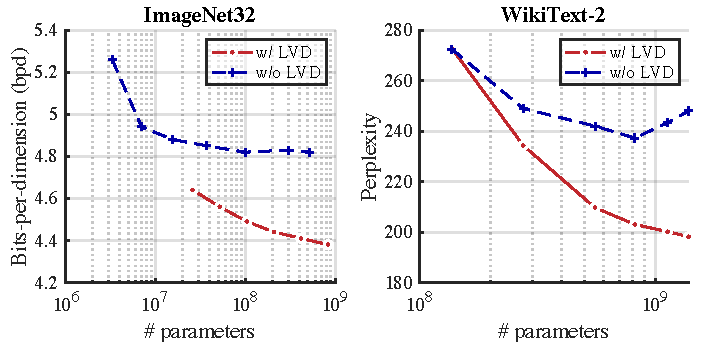
\includegraphics[width=0.6\columnwidth]{figures/fig-overview-results.pdf}
    \vspace{-2.0em}
    \caption{Latent variable (LV) distillation significantly boosts PC performance on challenging image (ImageNet32) and language (WikiText-2) modeling datasets. Lower is better.}
    \label{fig:overview-res}
    \vspace{-0.6em}
\end{wrapfigure}

The development of tractable probabilistic models~(TPMs) is an important task in machine learning: they allow various tractable probabilistic inference (e.g., computing marginal probabilities), enabling a wide range of down-stream applications such as lossless compression~\citep{liu2022lossless} and constrained/conditional generation~\citep{peharz2020einsum}. Probabilistic circuit~(PC) is a unified framework for a wide range of families of TPMs, examples include bounded tree-width graphical models~\citep{meila2000learning}, And-Or search spaces~\citep{marinescu2005and}, hidden Markov models~\citep{rabiner1986introduction}, Probabilistic Sentential Decision Diagrams~\citep{kisa2014probabilistic} and sum-product networks~\citep{poon2011sum}. Yet, despite the tractability of PCs, scaling them up for generative modeling on large and high-dimensional vision/language dataset has been a key challenge. 
% \guy{make sure to cite other PC labs, not just UCLA}

% \guy{make this a bit more dramatic by saying that recent progress in PC learning on GPUs (Einets, Juice/HCLTs) has made it possible to scale such models to X million parameters. Yet these computational breakthroughs are not leading to the expected large-scale learning breakthroughs.}

By leveraging the computation power of modern GPUs, recently developed PC learning frameworks \citep{peharz2020einsum,molina2019spflow,dang2021juice} have made it possible to train PCs with over 100M parameters (\eg \citet{correia2022continuous}). Yet these computational breakthroughs are not leading to the expected large-scale learning breakthroughs: as we scale up PCs, their performance immediately plateaus~(dashed curves in Fig.~\ref{fig:overview-res}), even though their actual expressive power should increase monotonically with respect to the number of parameters. Such a phenomenon suggests that the existing optimizers fail to utilize the expressive power provided by large PCs. PCs can be viewed as latent variable models with a deep hierarchy of latent variables. As we scale them up, size of their latent space increases significantly, rendering the landscale of the marginal likelihood over observed variables highly complex.
% and the EM algorithms alternate between inferring the assignments to latent variables~(E-step) and maximizing training log-likelihood by re-estimating PC parameters \wrt the assignments to latents~(M-step); though the M-step is guaranteed to improve model performance, we hypothesize that the E-step can easily ``stuck" at local optima due to bad random initialization.
% \guy{not sure if it's wise to make this EM specific. Someone can always say: just do SGD on the likelihood. I think we want to say that the marginal likelihood landscape is complex, the model is deep, etc., which someone means existing optimizers struggle to scale to vast amounts of latent variables.} \guy{Thinking about it more, the E step getting stuck actually makes no sense. Both the E step and the M step are exact in EM. It's just that they optimize a lower bound on the marginal likelihood that can be stuck in a local optimum} 
We propose to ease this optimization bottleneck by \textbf{latent variable distillation}~(LVD):~we provide extra supervision to PC optimizers by leveraging less-tractable yet more expressive deep generative models to induce semantics-aware assignments to the latent variables of PCs, in addition to the observed variables. 

The LVD pipeline consists of two major components: (i)~inducing assignments to a subset of~(or all) latent variables in a PC by information obtained from deep generative models and (ii)~estimating PC parameters given the latent variable assignments. For~(i), we focus on a clustering-based approach throughout this paper: we cluster training examples based on their neural embeddings and assign the same values to latent variables for examples in the same cluster; yet, we note that there is no constraint on how we should assign values to latent variables and the methodology may be engineered depending on the nature of the dataset and the architecture of PC and deep generative model. For~(ii), to leverage the supervision provided by the latent variable assignments obtained in~(i), instead of directly optimizing the maximum-likelihood estimation objective for PC training, we estimate PC parameters by optimizing the its lower-bound shown on the right-hand side:
    \begin{align}
        {\sum}_{i=1}^{N} \log \p(\x^{(i)}) := {\sum}_{i=1}^{N}\log{\sum}_{\z} \p(\x^{(i)}, \z) \geq {\sum}_{i=1}^{N} \log\p(\x^{(i)}, \z^{(i)}), 
        \label{eq:mle-lowerbound}
    \end{align}
where $\{\x^{(i)}\}_{i=1}^{N}$ is the training set and $\z^{(i)}$ is the induced assignments to the latent variables for $\x^{(i)}$. After LVD, we continue to finetune PC on the training examples to optimize the actual MLE objective, \ie ${\sum}_{i} \log \p(\x^{(i)})$. 

As shown in Figure~\ref{fig:overview-res}, with LVD, PCs successfully escape the plateau: their performance improves progressively as the number of parameters increases. Throughout the paper, we highlight two key advantages of LVD: first, it makes much better use of the extra capacity provided by large PCs; second, by leveraging the supervision from distilled LV assignments, we can significantly speed up the training pipeline, opening up possibilities to further scale up PCs.

% Moreover, this work paves the way towards a better integration of learning and reasoning by simultaneously leveraging the scalability of modern generative models and the tractability of PCs.

% To motivate and illustrate the intuition behind LV distillation, 
We start by presenting a simple example where we apply LVD on hidden Markov models to improve their performance on language modeling benchmarks~(Sec.~\ref{sec:hmm}). Then we introduce the basics for PCs~(Sec.~\ref{sec:pc}) and present the general framework of LVD for PCs~(Sec.~\ref{sec:lv-distillation}). The general framework is then elaborated in further details, focusing on techniques to speed up the training pipeline (Sec.~\ref{sec:efficient-pc-learning}).
In Section~\ref{sec:extracting-lvs}, we demonstrate how this general algorithm specializes to train patch-based PCs for image modeling. Empirical results show that LVD outperforms SoTA TPM baselines by a large margin on challenging image modeling tasks. Besides, PCs with LVD also achieve competitive results against various widely-used deep generative models, including flow-based models~\citep{kingma2018glow, dinh2016density} and variational autoencoders~\citep{maaloe2019biva}~(Sec.~\ref{sec:exp}).

% Probabilistic modeling is an important task in machine learning. Scaling up such models is a key challenge: probabilistic inference quickly becomes intractable as the models become large and sophisticated~\cite{roth1996hardness}. Central to this effort is the development of \emph{tractable probabilistic models} (TPMs) that guarantee tractable probabilistic inference in the size of the model, yet can efficiently represent a wide range of probability distributions. There has been a proliferation of different classes of TPMs. Examples include bounded-treewidth graphical models~\citep{meila2000learning}, determinantal point processes~\citep{borodin2005eynard,MAL-044}, and various probabilistic circuits~\citep{darwiche2009modeling,kisa2014probabilistic,AAAI-Tutorial} such as sum-product~networks~\citep{poon2011sum}.

% One key challenge for scaling PC models to large and high-dimensional dataset lies in the difficulty of optimization: as shown in Figure~\ref{fig:teaser}, even though the expressive power of the PC models should increase as the \# of parameters increases, their performance on the language/image modeling benchmarks quickly reaches a bottleneck. Such phenomenon suggests that the expectation-maximization (EM) algorithm for training PCs fail to utilize the expressive power provided by the extra parameters. The EM algorithm alternates between inferring the assignments to latent variable (E-step) and estimating parameters (M-step). The E-step XXX.

% We first illustrate our intuition via HMM and preliminary experiments show that warm-up effectively overcome the bottleneck of scaling PCs~(Sec.~\ref{sec:case-study}). Then we show that such idea can be generalized to arbitrary PCs and. 

% What we propose in this paper should be viewed as a general framework rather than a specific algorithm: (i) it is very general and can be applied to any PC models yet (ii) the actual choice of latent variables and methods for estimating values of latent values should be engineered based on the specific applications. The empirical results shown in our paper provide strong  

% In Section~\ref{sec:case-study}, we use HMM as an illustrating example to show the intuition a for PC warm-up. We introduce the basics for PCs in Section~\ref{sec:background} and describe the general PC warm-up pipeline in Section~\ref{sec:warmup}. In Section~\ref{sec:patch-model}, we describe the construction and warm-up procedure of a specific PC architecture for image modeling. 


% Empowered by various neural architectures, deep generative models have achieved remarkable performance on modeling visual and textual data. Yet, the number of ways we can query DGMs is limited: GPT-3 only supports computation of next token given prefix XXX . This motivates the development of tractable probabilistic models (TPMs) that supports more tractable queries (e.g. marginal/MAP infrence). Examples of TPMs include XXX. PCs XXX. However, PCs suffer from the issue of scalability; in particular, as shown in Figure~\ref{fig:teaser}, even though the expressive power of HMM/HCLT should increase as the number of parameters increase, the actual performance does not, suggesting that the EM optimization suffers from XXX. In this work, through two examples: , we propose a general framework to overcome. In the M-step, we estimate parameters given XXX is easy; in the E-step, we're supposed to estimate latent variable assignment given the current model. In image/language modeling, (partial) assignment to latent variables can also be inferred from neural information.

% In latent variable models, we can 

% Assume there exists some f such that f(x) gives meaning assignment to LVs given an example, we can optimize XXX.

\section{Latent Variable Distillation for Hidden Markov Model}
\label{sec:hmm}
In this section, we consider the task of language modeling by hidden Markov models~(HMM) as an illustrating example for LVD. In particular, we demonstrate how we can use the BERT model~\citep{devlin2019bert} to induce semantics-aware assignments to the latent variables of HMMs. Experiments on the WikiText-2~\citep{merity2016pointer} dataset show that our approach effectively boosts the performance of HMMs compared to their counterpart trained with only random initialization.

\paragraph{Dataset \& Model.} The WikiText-2 dataset consists of roughly 2 million tokens extracted from Wikipedia, with a vocabulary size of 33278. Following prior works on autoregressive language modeling~\citep{radford2019language}, we fix the size of the \emph{context window} to be 32: that is, the HMM model will only be trained on subsequences of length 32 and whenever predicting the next token, the model is only conditioned on the previous 31 tokens. In particular, we adopt a \emph{non-homogeneous} HMM model, that is, its transition and emission probabilities at each position share no parameters; Figure~\ref{fig:hmm}) shows its representation as a graphical model, where $X_i$s are the observed variables and $Z_i$s are the latent variables.
To facilitate training and evaluation, we pre-process the tokens from WikiText-2 by concatenating them into one giant token sequence and collect all subsequences of length $32$ to construct the train, validation and test sets, respectively.

\begin{figure}
     \centering
     \begin{subfigure}[b]{0.27\textwidth}
         \centering
         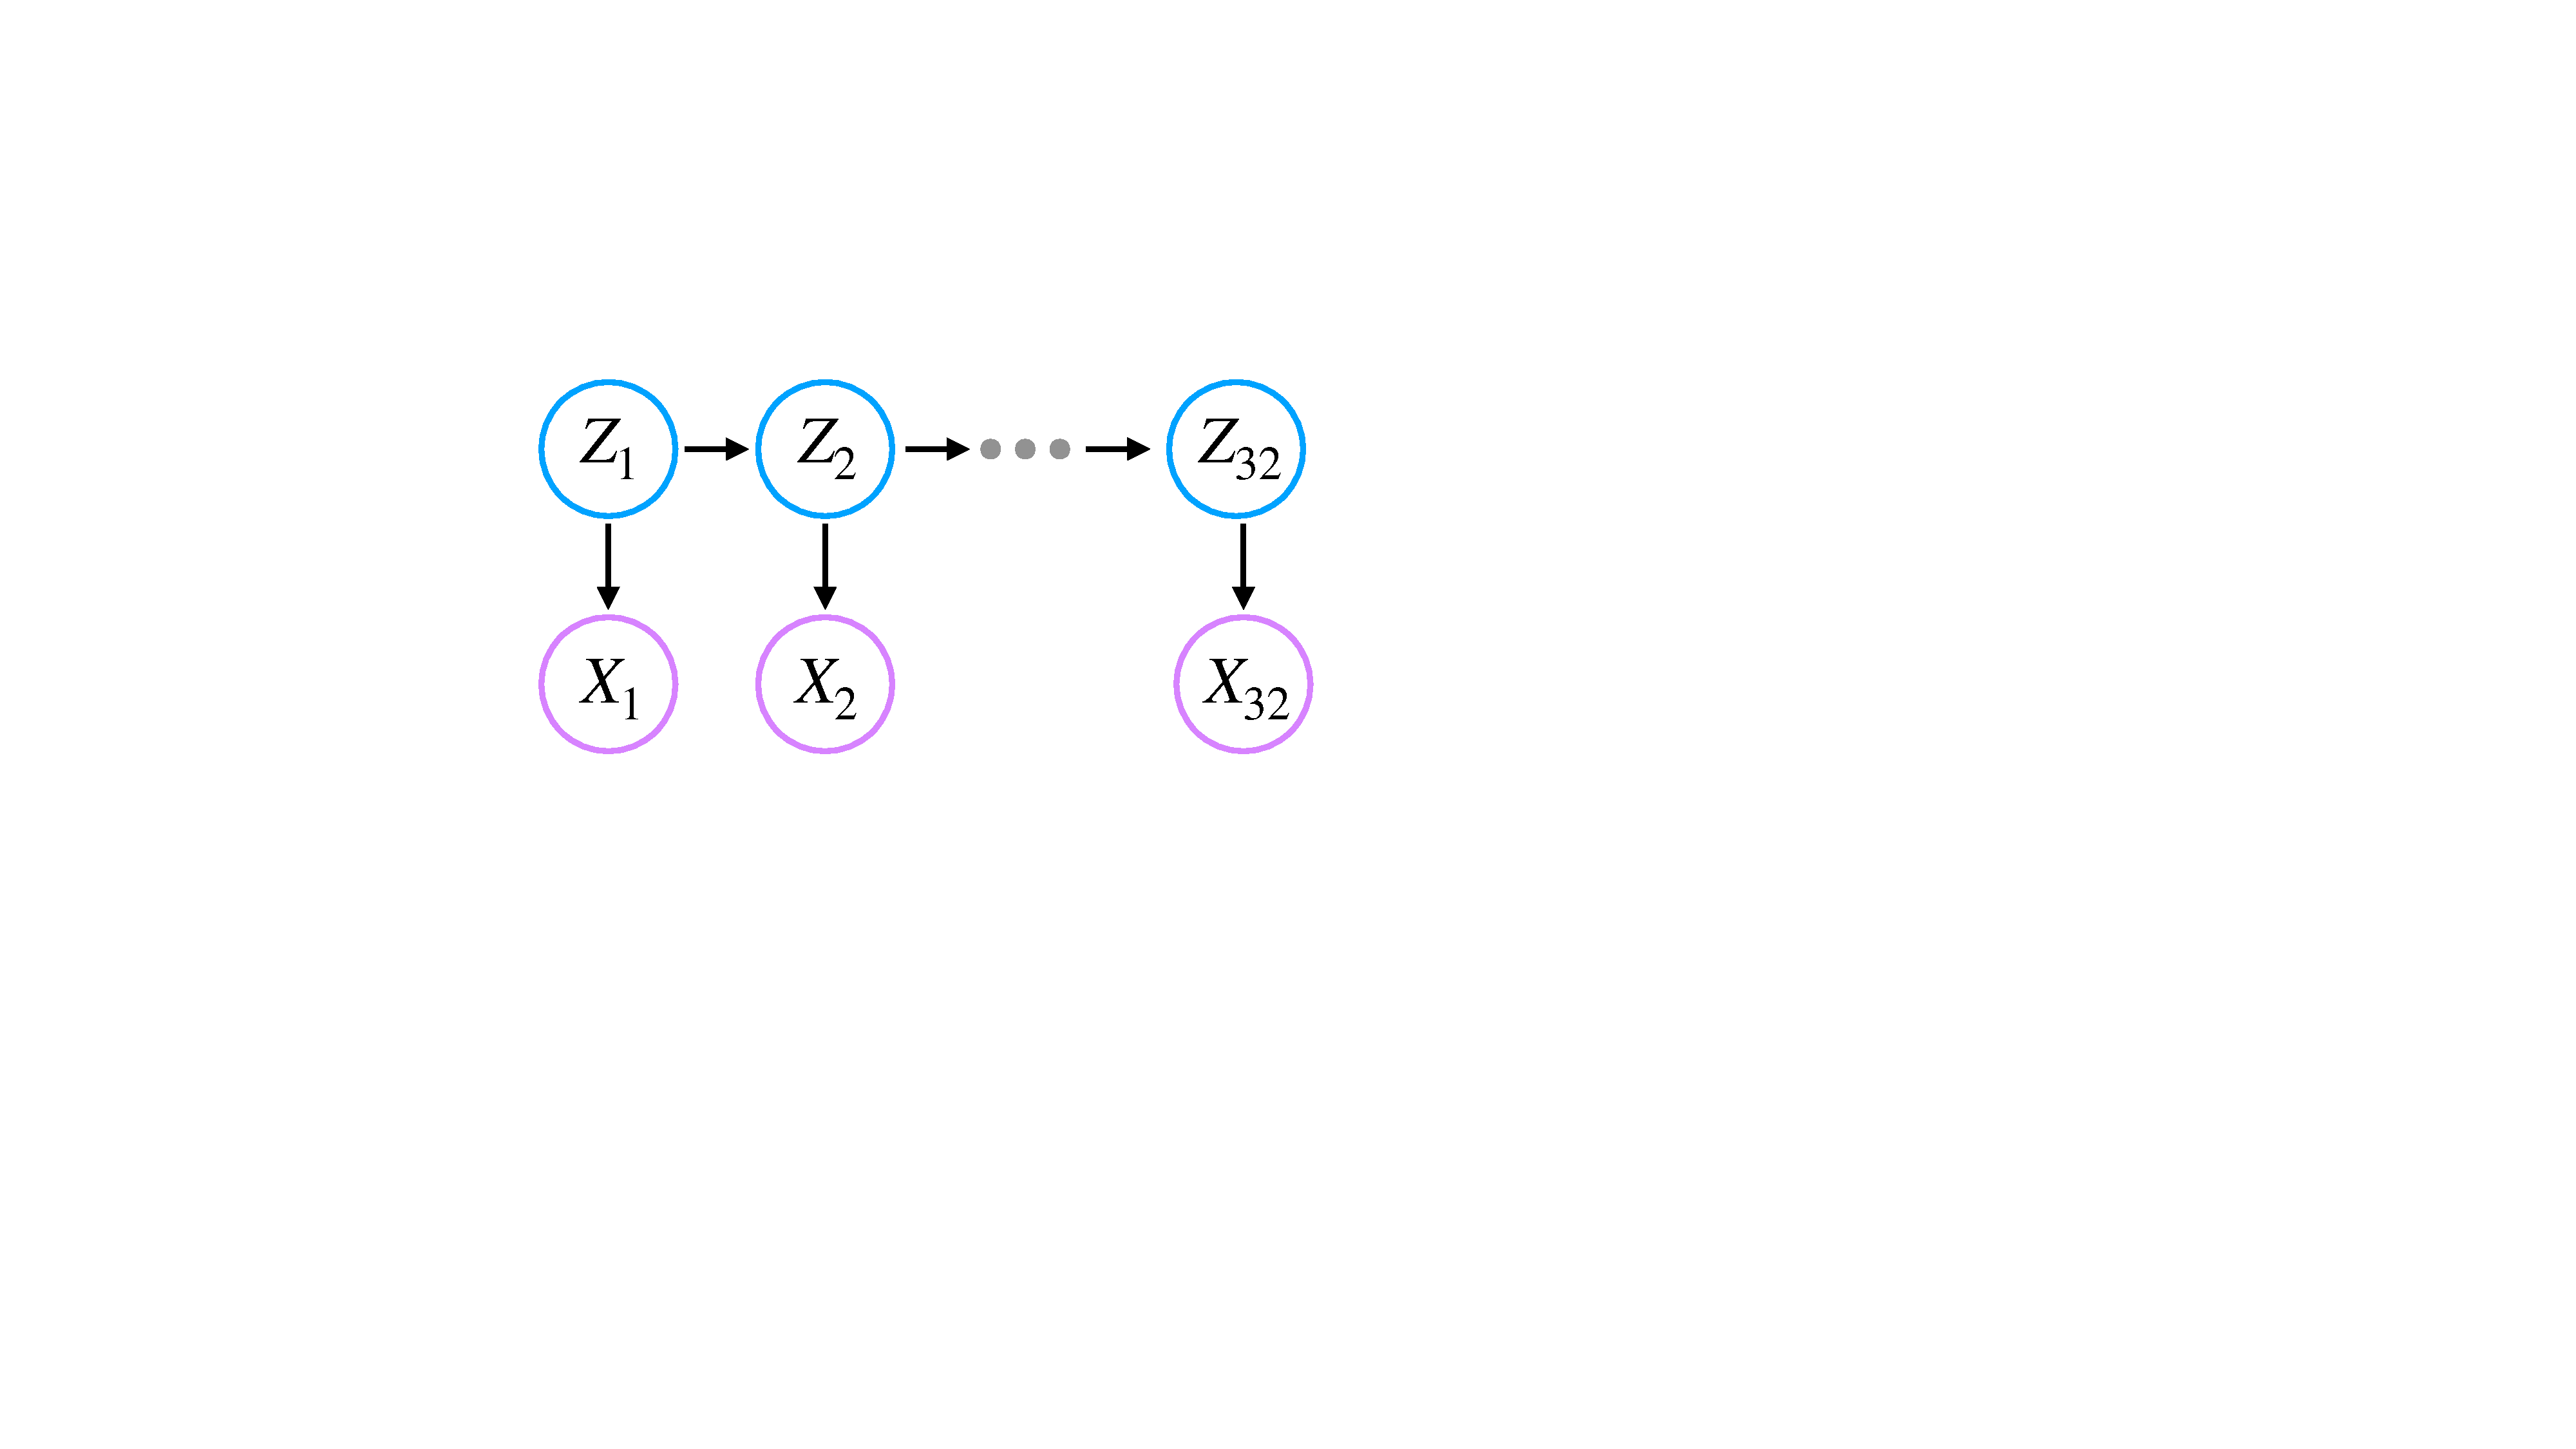
\includegraphics[width=\textwidth]{figures/hmm.pdf}
         \hfill\\
         \hfill\\
         \hfill\\
         \hfill\\
         \caption{Graphical model representation of an HMM modeling token sequences of length 32. $X_{i}$ are the observed variables and $Z_{i}$ are the latent variables.}
         \label{fig:hmm}
     \end{subfigure}
     ~\hfill
     \begin{subfigure}[b]{0.68\textwidth}
         \centering
         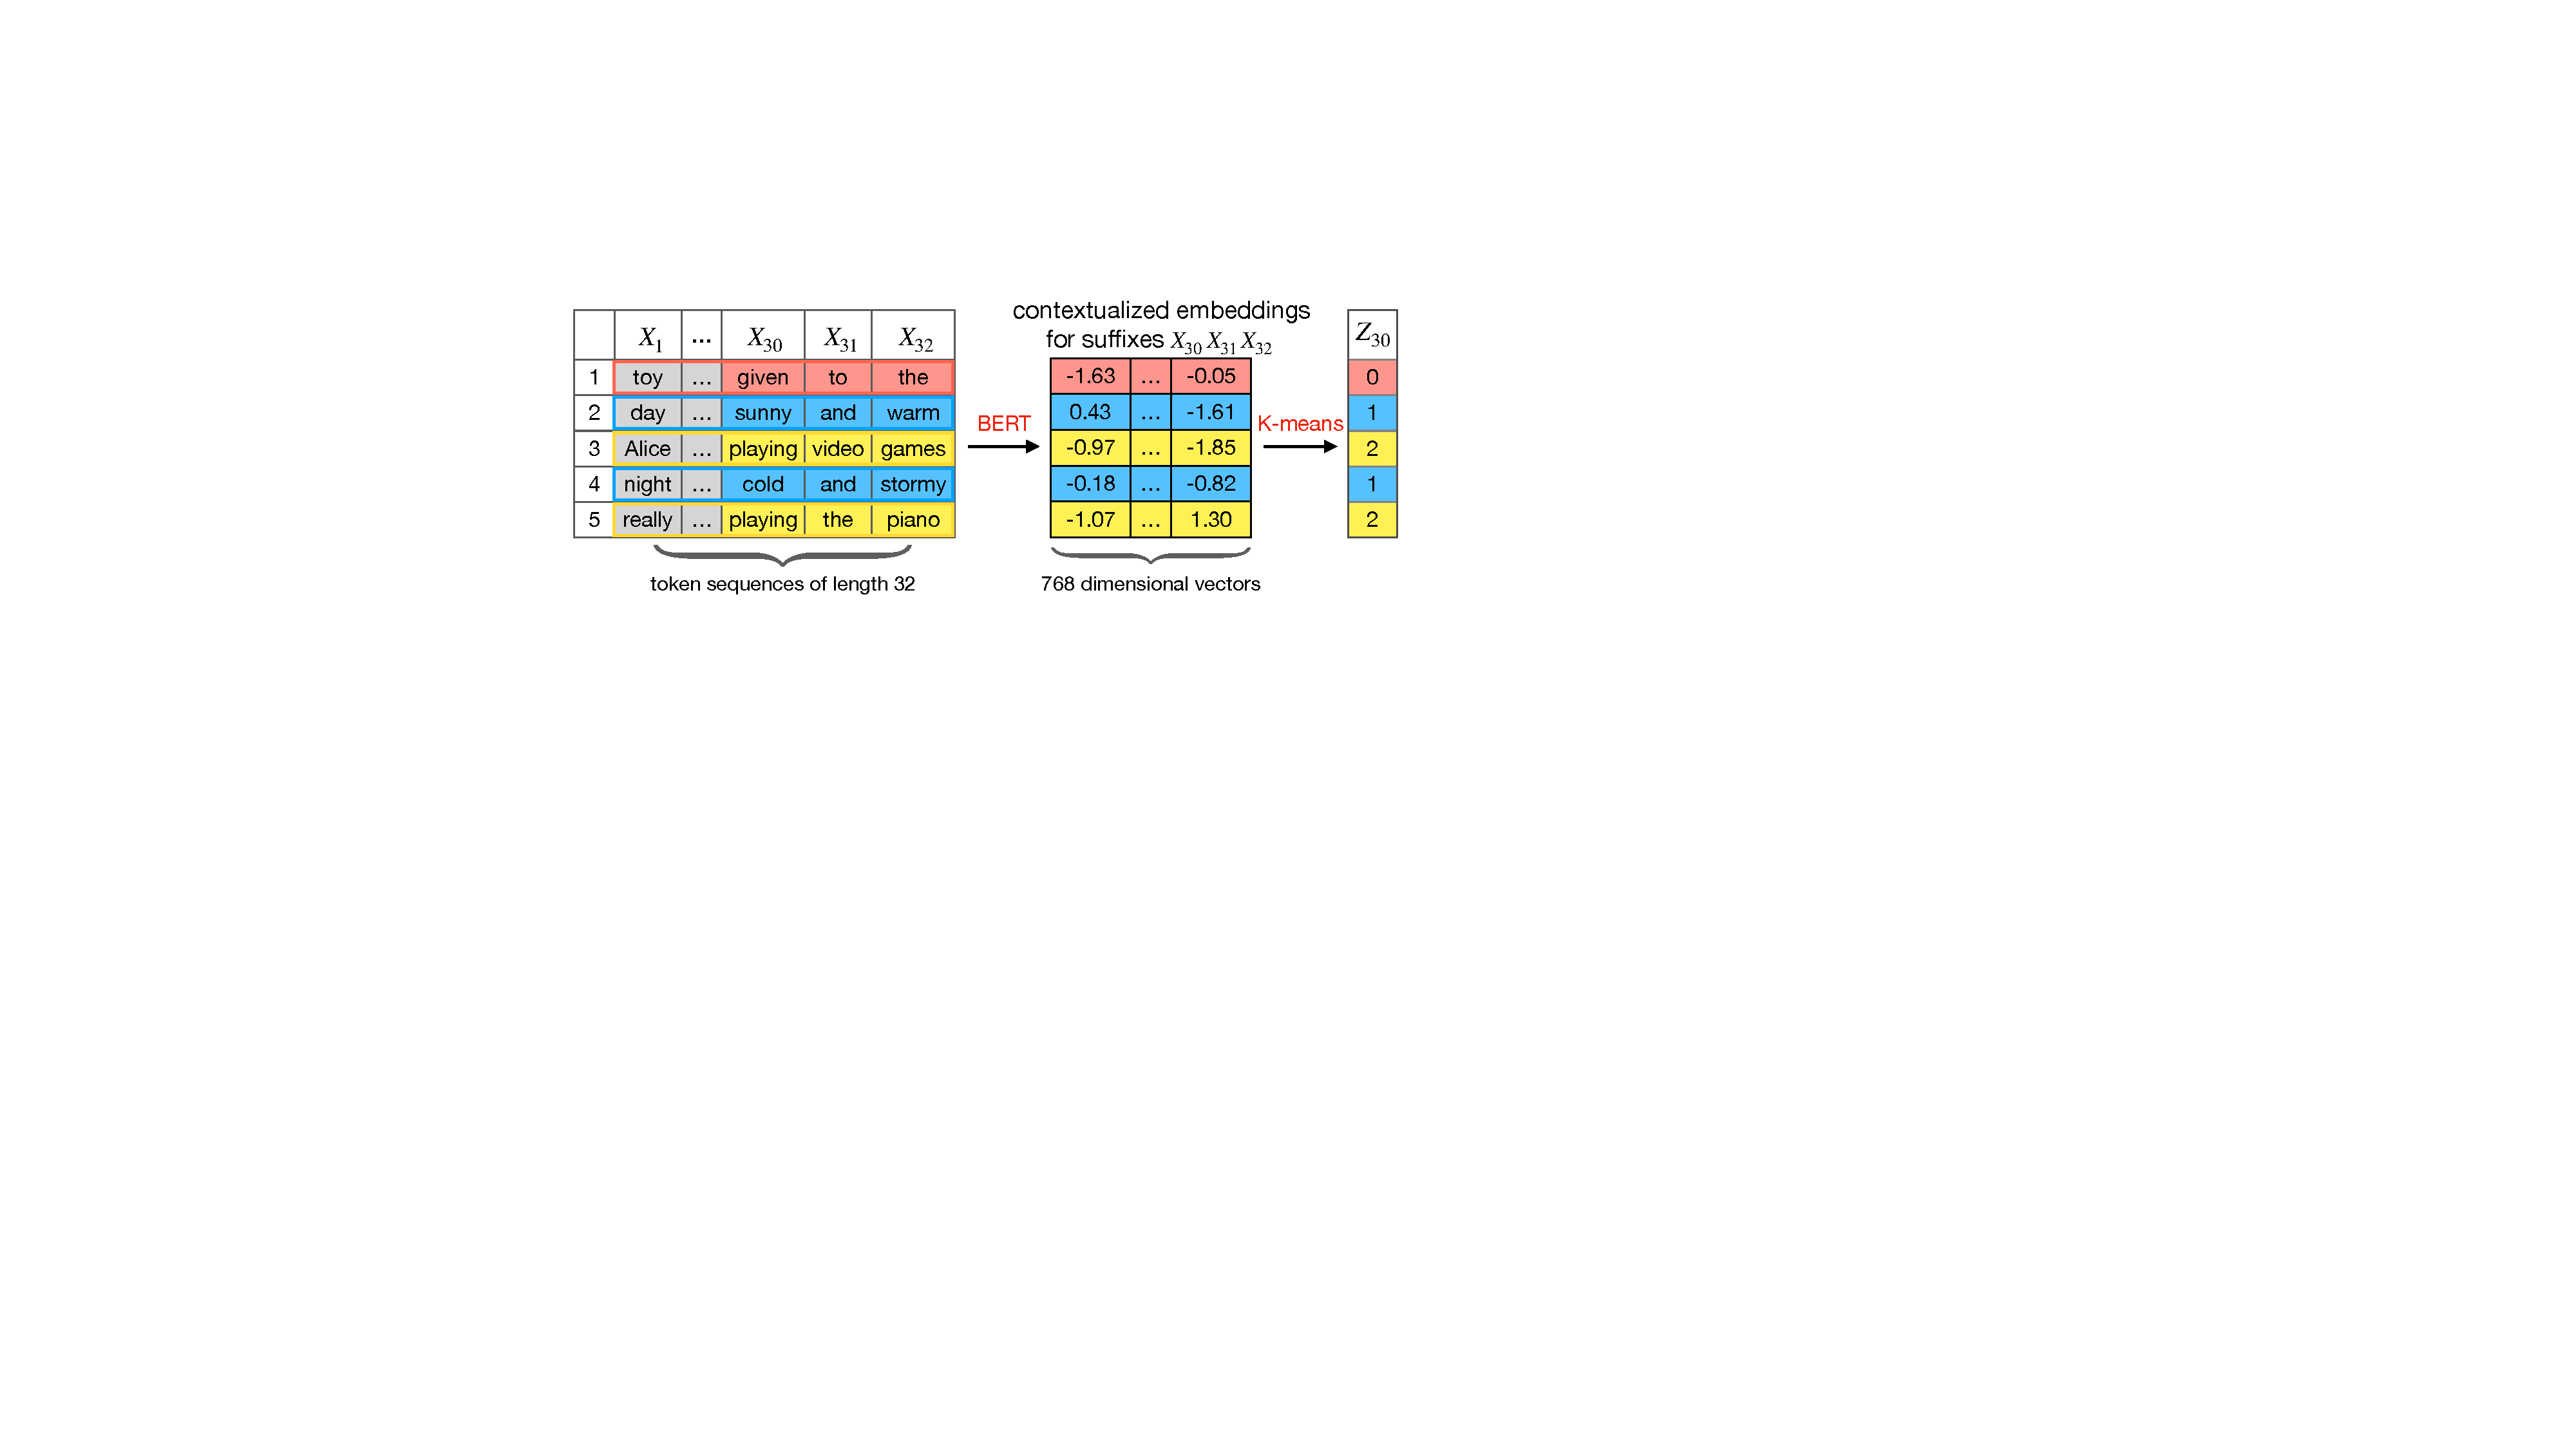
\includegraphics[width=\textwidth]{figures/hmm-warmup.pdf}
         \caption{Pipeline for inferring values for one latent variable $Z_{30}$. We feed token sequences to the BERT model to obtain contextualized embeddings for their suffixes $X_{30}X_{31}X_{32}$; then we cluster all suffix embeddings into $h$ clusters; here $h = 3$ is the number of hidden states and the value for $Z_{30}$ is set to the cluster id. We repeat this procedure \emph{independently} to infer values for all $Z_i$s.}
         \label{fig:hmm-warmup-pipeline}
     \end{subfigure}
        \caption{Latent variable distillation pipeline for hidden Markov models.}
        \label{fig:hmm-warmup}
\end{figure}
% For the training set, we concatenate all items to form one string $S$ and let $D_{\text{train}} = \{s_i : s_i \text{a substring of } S \text{ of length } 32\}$; similarly for the validation and test set. Our model is a non-homogeneous HMM of fixed length $32$, that is, the transition and emission probabilities share no parameters and could be different at each position. The observed variables are $X_{1}, \cdots, X_{32}$ and the latent variables are $Z_{1}, \cdots, Z_{32}$.


\paragraph{Latent Variable Distillation.} Let $\data \!=\! \{\x^{(i)}\}_{i}$ be the training set; Figure~\ref{fig:hmm-warmup} shows an example on how to induce, for each training example $\x^{(i)}$, its corresponding assignment to the latent variable $Z_{30}$. We first feed all training examples to the BERT model to compute the contextualized embeddings for their suffixes $X_{30}X_{31}X_{32}$.
% which is the average of the contextualized token embeddings in the suffix. 
We cluster all suffix embeddings into $h$ clusters by the K-means algorithm~\citep{lloyd1982least}, where $h$ is the number of hidden states; then, we set $Z_{30}$ to be the cluster id of their corresponding suffixes, that is, suffixes in the same cluster get the same latent variable value:
% As exemplified in Figure 2, for the training examples {x(i)}i, we first feed them to the BERT model to obtain contextualized embeddings for their suffixes and cluster the embeddings by the K-means algorithm (Lloyd, 1982) algorithm~\citep{lloyd1982least}.
% \anji{Probably need to make it clear that we are computing the embeddings for the suffix of every $\x_i$. And the embeddings at each position are clustered separately, leading to $z_1, \dots, z_{32}$.}\anji{We may also want use \cref{fig:hmm-warmup} to provide more detailed examples.} 
% We then assign the same values to the latent variables: 
the intuition is that if the BERT embeddings of some suffixes are close to each other then the suffixes should be relatively similar, suggesting that they should be ``generated'' by the same hidden state. We repeat this procedure for 32 times to infer the values for all $Z_i$s. Now we obtain an ``augmented'' training set ${\data_{\mathrm{aug}}} = \{(\x^{(i)}, \z^{(i)})\}_{i}$, where $\z^{(i)}$ are the corresponding assignments to the latent variables $\Z$; then, as suggested by Equation~\ref{eq:mle-lowerbound}, we maximize the lower-bound $\sum_{i}\log\p(\x^{(i)}, \z^{(i)})$ for the true MLE objective $\sum_{i}\log\p(\x^{(i)})$. The parameters of the HMM that maximize $\sum_{i} \log \p(\x^{(i)}, \z^{(i)})$, denoted by $\mathbf{\theta}^{*}$, can be solved in closed-form. Finally, using $\mathbf{\theta}^{*}$ as a starting point, we finetune the HMM model via EM to maximize the true MLE objective $\sum_{i}\log\p(\x^{(i)})$. 

\paragraph{Experiments.}
We apply LVD to HMMs with a varying number of hidden states $h$ = $128$, $256$, $512$, $750$, $1024$ and $1250$; for comparison, we also train HMMs with random initialization. Please refer to \cref{sec:exp-details} for details about training. The plot on the right of Figure~\ref{fig:overview-res} shows the test perplexity of HMMs~(w/ and w/o LVD) on WikiText-2: as the number of parameters in HMM increases, the performance of the HMMs trained with random parameter initialization immediately plateaus, while the performance of the HMMs trained with LVD progressively improves, suggesting that LVD effectively exploits the express power of the larger models.

% In this section, we use hidden Markov model (HMM) as an illustrating example to show how neural embeddings can be used to guide XXX. Specifically, we 
% We consider the task of language modeling on the WikiText-2 benchmark; specifically, we concatenate all items into one string $S$ and let 
% Given a training set $D_{\text{train}} = \{s_i\}_{1\leq i \leq m}$ consisting of $m$ examples of length $n$, the maximum likelihood estimation (MLE) objective is given by:
% \begin{align*}
%  &\argmax_{\theta} \prod_{i}{\Pr}_{\theta}(X_1 = s_{i,1}, \cdots, X_n = s_{i,n}) \\
% & = \argmax_{\theta} \prod_{i} \sum_{z_1, \cdots, z_n} {\Pr}(X_1 = s_{i, 1}, \cdots, X_n = s_{i, n}, Z_1 = z_1, \cdots, Z_n = z_n) \\
% & = \prod_{i} \sum_{z_1, \cdots, z_n} \prod_{j} {\Pr}(X_j = s_{i, j} \given Z_j = z_j) \prod_{j} {\Pr}(Z_{j+1} = z_{j+1} \given Z_j = z_j) {\Pr}(Z_1 = z_1)
% \end{align*}

% \begin{align*}
% {\Pr}(Z_1 = c_{i,1})\prod_{1\leq j < n} {\Pr}(Z_{j+1} = c_{i,j+1} \given Z_j = c_{i,j})\prod_{1\leq j < n} {\Pr}(X_j = s_{i, j} \given Z_j = c_{i,j})
% \end{align*}
% where $c_{i,j}$ is the value assigned to the latent variable $Z_j$ for example $s_i$.

% \anji{I think we may want this section to be less technical and more intuitive. Maybe we can achieve this by saying there are the transition and emission parts in a HMM. And describe how the parameters of both parts can be obtained from BERT, \ie, what are the ``transition part'' and ``emission part'' in BERT.}

% \anji{Maybe end this section with the question: how this high-level idea can be applied to a broader class of TPMs? In the following, we introduce the warmup idea in the context of PCs, a general TPM model.}

% \section{Latent Variable Distillation for Probabilistic Circuits}

% \section{Image Modeling }

% \subsection{Extracting LVs from Expressive Generative Models}

% \subsection{Parameter Learning with Latent Variable Supervision}

% \subsection{Experiments}

\section{Latent Variable Distillation for Probabilistic Circuits}
\label{sec:background}

The previous section uses HMM as a specific TPM to elaborate key steps in LVD. In order to generalize LVD to broader TPMs, this section introduces Probabilistic Circuit (PC), which is a unifying framework for a large collection of tractable probabilistic models.
% , examples include hidden Markov models~(HMMs), Sum-Product Networks~(SPNs)~\citep{poon2011sum}, And-Or search spaces~\citep{marinescu2005and}, and Probabilistic Sentential Decision Diagrams~(PSDDs)~\citep{kisa2014probabilistic}.
% \guy{but also HMMs}

\subsection{Probabilistic Circuits: A General TPM Framework}
\label{sec:pc}

PCs represent distributions as deep computation graphs;

\begin{defn}[Probabilistic Circuits]
\label{def:pc}
A PC $\p(\X)$ that encodes a distribution over variables $\X$ is defined by a parameterized directed acyclic computation graph (DAG) with a single root node $n_r$. Every node in the DAG corresponds to a computational unit. Specifically, every leaf node is defined by an \emph{input unit} and every inner node $n$ represents either a \emph{sum} or \emph{product unit} that receives inputs from its children, termed $\ch(n)$. Each PC unit $n$ encodes a distribution $\p_{n}$:
    \begin{align}
        % \setlength{\abovedisplayskip}{-0.8em}
        % \setlength{\belowdisplayskip}{-1.6em}
        \p_{n} (\x) := \begin{cases}
            f_{n} (\x) & \text{if~}n\text{~is~an~input~unit}, \\
            \sum_{c \in \ch(n)} \theta_{c\given n} \cdot \p_{c} (\x) & \text{if~}n\text{~is~a~sum~unit}, \\
            \prod_{c \in \ch(n)} \p_{c} (\x) & \text{if~}n\text{~is~a~product~unit},
        \end{cases}
        \label{eq:pc-def}
    \end{align}
\noindent where $f_{n}(\x)$ is a univariate probability distribution (\eg Gaussian, Categorical) defined on a variable in $\X$ and $\theta_{c \given n}$ is the parameter corresponds to edge $(n, c)$. For every sum unit $n$, we assume all its edge parameters $\{\theta_{c \given n}\}_{c \in \ch(n)}$ are non-negative and sum up to one. Intuitively, a product unit encodes a factorized distribution over its inputs, and a sum unit models a weighted mixture of its children's distributions. A PC represents the distribution encoded by its root unit $n_r$. We further assume w.l.o.g. that PCs alternate between sum and product layers before reaching an input layer.
\end{defn}

A key property that separates PCs from many other generative models is their \emph{tractability}, \ie the ability to answer various queries exactly while efficiently. Such queries include common ones like marginals and conditional probabilities as well as task-specific ones such as structured prediction \citep{shao2022conditional} and variational inference \citep{shih2020probabilistic}. The tractability of PCs is governed by structural constraints on their DAG structure. For example, \emph{smoothness} and \emph{decomposability} together guarantee linear time (\wrt size of the PC) computation of arbitrary marginal probabilities.

\begin{defn}[Smoothness and Decomposability]
\label{def:sm-dec}
Define the (variable) scope $\scope(n)$ of a PC unit $n$ as the set of variables defined by all its descendent input units. A PC is smooth if for every sum unit $n$, all its children have the same scope: $\forall c_{1}, c_{2} \!\in\! \ch(n), \scope(c_{1}) \!=\! \scope(c_{2})$. A PC is decomposable if the children of every product unit $n$ have disjoint scopes: $\forall c_{1}, c_{2} \!\in\! \ch(n) (c_{1} \!\neq\! c_{2}), \scope(c_{1}) \cap \scope(c_{2}) \!=\! \emptyset$.
\end{defn}

\begin{figure}
    \centering
    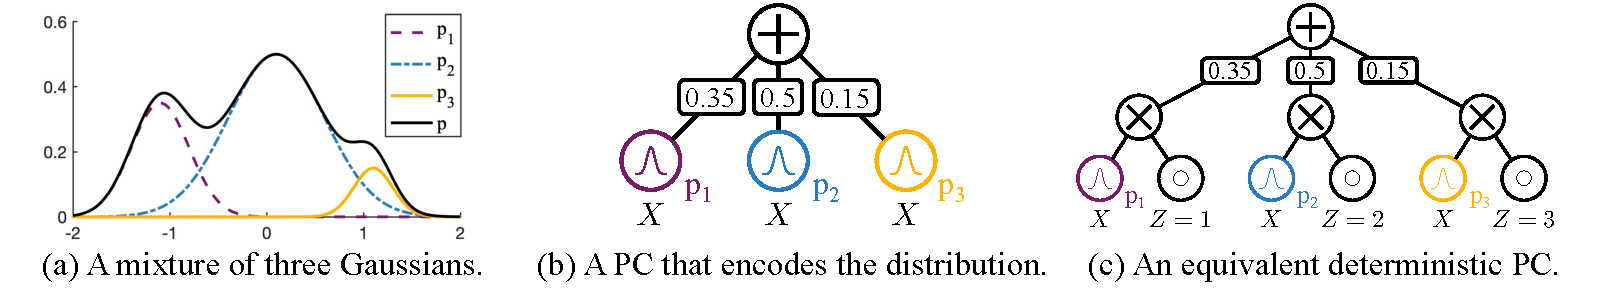
\includegraphics[width=\columnwidth]{figures/fig-mixture-of-gaussian.pdf}
    \vspace{-1.8em}
    \caption{A mixture-of-Gaussian distribution (a) and two PCs (b-c) that encode the distribution.}
    \label{fig:mixture-of-gaussian}
    \vspace{-1em}
\end{figure}

\subsection{Materializing and Distilling Latent Variables in Probabilistic Circuits}
\label{sec:lv-distillation}


% The expressiveness of PCs comes from the fact that they can be viewed as latent variable models with a deep hierarchy of latent variables (LVs) \citep{peharz2016latent,liu2021tractable}. 

PCs can be viewed as latent variable models with discrete latent spaces~\citep{peharz2016latent}. Specifically, since a sum unit in a PC can be viewed as a mixture over its input distributions, it can also be interpreted as a simple latent variable model $\sum_{\z} \p(\x \given z) \p(z)$, where $z$ decides which input to choose from and the summation enumerates over all inputs. \cref{fig:mixture-of-gaussian} shows such an example, where the sum unit in \cref{fig:mixture-of-gaussian}~(b) represents the mixture over Gaussians in \cref{fig:mixture-of-gaussian}~(a). 

In general, the latent space for large PCs is hierarchical and deeply nested; as we scale them up, we are in effect scaling up the size/complexity of their latent spaces, making it difficult for optimizers to find good local optima. To overcome such bottleneck, we generalize the idea presented in~\cref{sec:hmm} and propose \emph{latent variable distillation}~(LVD). The key intuition for LVD is to provide extra supervision on the latent variables of PCs by leveraging existing deep generative models: given a PC $\p(\X)$; we view it as a latent variable model ${\sum}_{\z}\p(\X, \Z=\z)$ over some set of latents $\Z$ and assume that for each training example $\x^{(i)}$, a deep generative model can always induce some semantics-aware assignment $\Z=\z^{(i)}$; then, instead of directly optimizing the MLE objective ${\sum}_{i}\log\p(\x^{(i)})$, we can optimize its lower-bound ${\sum}_{i}\log\p(\x^{(i)}, \z^{(i)})$, thus incorporating the guidance provided by the deep generative model. The LVD pipeline consists of three major steps, elaborated in the following:

% assume that we are given some deep generative model 
% Given a PC P and some choice of latent variables Z;and training set D, instead of directly optimizing LL(p, X), we optimize its lower-bound Pr(X, Z=z) 
% Instead of directly optimizing Pr(X), we optimize its Pr(X, Z) for some choice of latent variables Z, where we 
% The key intuition for LVD is to firstly materialize latent variables to obtain a new PC representing the joint distribution $\Pr(\X, \Z)$, where the latent variables $\Z$ are explicit and its marginal distribution $\Pr(\X)$ corresponds to the original PC. By introducing latent variables $\Z$, we can encode information from other deep generative models such as fine-tuned language or image embedding by mapping the embedding to latent variable $\Z$ parameters. By optimizing $\Pr(\X, \Z)$ via MLE and then marginalize $\Z$ out in the end, we can get a good lower bound for $\Pr(\X)$. 

% The LVD pipeline consists of three major steps, elaborated in the following:

\boldparagraph{Step 1: Materializing Latent Variables.}
The first step of LVD is to \emph{materialize} some/all latent variables in PCs. By materializing latent variables, we can obtain a new PC representing the joint distribution $\Pr(\X, \Z)$, where the latent variables $\Z$ are explicit and its marginal distribution $\Pr(\X)$ corresponds to the original PC. 
Although we can assign every sum unit in a PC an unique LV, the semantics of such materialized LVs depend heavily on PC structure and parameters, 
\begin{wrapfigure}{r}{0.5\columnwidth}
    \centering
    \vspace{-0.4em}
    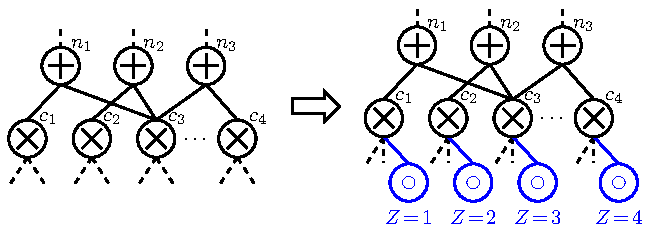
\includegraphics[width=0.5\columnwidth]{figures/fig-add-lvs.pdf}
    \vspace{-2.0em}
    \caption{Materializing LVs in a PC.}
    \label{fig:add-lvs}
    \vspace{-1.2em}
\end{wrapfigure}
which makes it extremely hard to obtain supervision. 
Instead, we choose to materialize LVs based on subsets of observed variables defined by a PC. That is, each materialized LV corresponds to all PC units with a particular variable scope (\cf Def.~\ref{def:sm-dec}). 
For example, we can materialize the latent variable $Z$, which corresponds to the scope $\scope(n_i)$ ($\forall i \!\in\! [3]$), to construct the PC in \cref{fig:mixture-of-gaussian}(c) that explicitly represents $\p(X, Z)$, whose marginal distribution $\p(X)$ corresponds to the PC in \cref{fig:mixture-of-gaussian}~(b). \cref{alg:lv}~\citep{peharz2016latent} provides one general way to materialize latent variables in PCs, where \cref{fig:add-lvs} shows an example where the four product units $c_1, \dots, c_4$ are augmented with input units $Z\!=\!1, \dots, Z\!=\!4$, respectively. 
% Let $\W$ be the scope of some existing unit in a PC $p(\X)$, \cref{alg:lv} describes how to materialize a categorical LV $Z$ corresponding to $\W$. We first collect all product units with scope $\W$ and form an (arbitrarily) ordered set $S_{\W}$~(line 3).
% Specifically, we first denote the set of product units with scope $\W$ as $S_{\W}$ and assign its elements an arbitrary order (line 3). 
% Without loss of generality, we can assume that sum and product units always alternate in~$p(\X)$~(\cf Def.~\ref{def:pc}) and it follows that for every sum unit $n$ with scope $\W$, its children must belong to $S_{\W}$. Therefore, to ensure all such sum units are deterministic, we only need to assign every product unit in $S_{\W}$ a different latent category of $Z$. That is, for the $j$th element in $S_{\W}$~(line 4), denoted $n_j$, we can augment $n_j$ with an input unit $Z_i \!=\! j$ (line 5). As an example, the four product units $\{c_i\}_{i=1}^{4}$ in \cref{fig:add-lvs} are augmented with input units $Z\!=\!1, \dots, Z\!=\!4$, respectively. 
% This enforces determinism of $\{n_i\}_{i=1}^{3}$ since by choosing any specific value of $Z$, for any input assignment, sum units $\{n_i\}_{i=1}^{3}$ have at most one child with non-zero probability.

Continuing with our example in \cref{fig:mixture-of-gaussian}, note that after materialization, the sum unit representing $\p(X, Z)$ in \cref{fig:mixture-of-gaussian}(c) is no longer a latent variable distribution: each assignment to $X, Z$ \emph{uniquely} determines the input distribution to choose, where the other inputs give zero probability under this assignment; we say that this sum unit is \emph{deterministic}~\citep{darwiche2003differential}.
\begin{defn}[Determinism]
Define $\supp(n)$ as the set of complete assignments $\x \!\in\! \val(\X)$ such that $\p_{n}(\x) \!>\! 0$. A sum unit $n$ is deterministic if its children have disjoint supports: $\forall c_1, c_2 \!\in\! \ch(n) (c_1 \!\neq\! c_2), \supp(c_1) \cap \supp(c_2) \!=\! \emptyset$. 
% A PC is deterministic if all its sum units are deterministic.
\end{defn}
Determinism characterizes whether a sum unit introduces latent variables: by materializing some sum units with the scope, we enforce them to become deterministic. Intuitively, more deterministic sum units in PCs implies smaller latent spaces, which implies easier optimization; in fact, if all sum units in a PC are deterministic then the MLE solution can be computed in closed-form~\citep{kisa2014probabilistic}. By materializing more latent variables, we make PCs ``more deterministic'', pushing the optimization procedure towards a closed-form estimation.

% Meanwhile, we never sacrifice model expressiveness since we are still training the original PC with potentially complex latent space. 
% LV distillation offers a solution to this dilemma: optimizing the lower-bound $\log \p(\x^{(i)}, \z^{(i)})$ (cf. Eq.~\ref{eq:mle-lowerbound}) of the marginal log-likelihood over the observed variables can be viewed as learning a PC over $\X$ and $\Z$, but with much fewer latent variables (\ie the ones that are not yet materialized). 
\begin{figure}[t]
\begin{algorithm}[H]
\caption{Materializing a LV in a PC 
% \guy{I believe this algorithm implicitly assumes structured decomposability, because if there are branches that do not decompose the scope into W exactly, then those will not have a Z and that will violate smoothness}
}
\label{alg:lv}
{\fontsize{9}{9} \selectfont
\begin{algorithmic}[1]

\STATE {\bfseries Input:} A PC $\p(\X)$ and a variable scope $\W$ for some sum unit in $\p(\X)$

\STATE {\bfseries Output:} An augmented PC $\p$ defined over $\{\X, Z\}$, where $Z$ is the materialized LV corresponding to $\W$

\STATE $S_{\W} \leftarrow \{n : n \in \p \text{~s.t.~} n \text{~is~a~product~unit~and~} \scope(n) = \W \}$ \hfill \textcolor[RGB]{115,119,123}{$\triangleright$ Created as an ordered set}

\FOR{\tikzmarknode{a1}{} $\! j = 1$ \textbf{to} $\abs{S_{\W}}$}
\STATE Let $n_j$ be the $j$th unit in $S_{\mathbf{W}}$
\STATE Add an input unit $c$ over $Z_i$ with distribution $\p_c(z_i) = \begin{cases} 1 & z_i = j, \\ 0 & \text{otherwise} \end{cases}$ as a new child of $n_j$

\ENDFOR

\end{algorithmic}
}
\end{algorithm}
\begin{tikzpicture}[overlay,remember picture]
    \draw[black,line width=0.6pt] ([xshift=-12pt,yshift=-3pt]a1.west) -- ([xshift=-12pt,yshift=-24pt]a1.west) -- ([xshift=-8pt,yshift=-24pt]a1.west);
\end{tikzpicture}
\vspace{-3em}
\end{figure}

\boldparagraph{Step 2: Inducing Latent Variable Assignments.}
Latent variable materialization itself cannot provide any extra supervision to the PC training pipeline; in addition, we also need to leverage some existing deep generative models to induce semantics-aware assignments for the materialized latent variables. Though there is no general guideline on how the assignments should be induced, we focus on a clustering-based approach throughout this paper. Recall from \cref{sec:hmm}, where we cluster the suffix embeddings generated by the BERT model and for each training example, we assign the latents the cluster id that its suffixes belong to. Similarly, for image modeling, in \cref{sec:extracting-lvs}, we will show how to induce latent variable assignments by clustering the embeddings for patches of images. The main take-away is that the method for inducing latent variable assignments should be engineered depending on the nature of the dataset and the architecture of PC and deep generative model.

% \anji{TODO: smooth transition sentences} \cref{alg:warmup} formalizes the complete PC warmup algorithm, which consists of three main steps. First, in lines 3-4, the algorithm materializes LVs specified by the variable partition $\{\X_i\}_{i=1}^{k}$ using \cref{alg:lv}. Next, we obtain LV assignments from the generative model and construct an augmented dataset $\data_{\mathrm{aug}}$ that additionally contains the induced assignments to LVs for each sample (line 5). \textsf{get\_latents} is used to extract LVs $\z$ from input $\x$, and will be described in \cref{sec:extracting-lvs}. Finally, in lines 6-8, the PC parameters are optimized by the above-described algorithm using $\data_{\mathrm{aug}}$ and $\data$. After warmup, we can remove the materialized LVs by deleting all input units correspond to variables in $\Z$.

\boldparagraph{Step 3: PC Parameter Learning.} 
Given a PC $\p(\X; \theta)$ with parameters $\theta$ and a training set $\data = \{\x^{(i)}\}$; in Step~1, by materializing some set of latent variables $\Z$, we obtain an augmented PC $\p_{\text{aug}}(\X, \Z; \theta)$ whose marginal distribution on $\X$ corresponds to $\p(\X; \theta$); in Step~2, by leveraging some deep generative model $\mathcal{G}$, we obtain an augmented training set $\data_{\text{aug}} = \{(\x^{(i)}, \z^{(i)})\}$. Note that since $\p_{\text{aug}}$ and $\p$ share the same parameter space, we can optimize ${\sum}_{i=1}^{N} \log\p_{\text{aug}}(\x^{(i)}, \z^{(i)}; \theta)$ as a lower-bound for ${\sum}_{i=1}^{N} \log \p(\x^{(i)}; \theta)$:
\begin{align*}
        {\sum}_{i=1}^{N} \log \p(\x^{(i)}; \theta) = 
        {\sum}_{i=1}^{N}\log{\sum}_{\z} \p_{\text{aug}}(\x^{(i)}, \z; \theta) \geq
        {\sum}_{i=1}^{N} \log\p_{\text{aug}}(\x^{(i)}, \z^{(i)}; \theta);
\end{align*}
we denote the parameters for $\p_{\text{aug}}$ after optimization by $\theta^{*}$. Finally, we initialize $\p$ with $\theta^{*}$ and optimize the true MLE objective with respect to the original dataset $\data$, ${\sum}_{i=1}^{N} \log \p(\x^{(i)}; \theta)$.

\boldparagraph{Summary.} Here we summarize the general pipeline for latent variable distillation. Assume that we are given: a PC $p(\X; \theta)$ over observed variables $\X$ with parameter $\theta$, a training set $\data = \{\x^{(i)}\}$ and a deep generative model $\mathcal{G}$:
\begin{enumerate}
    \item Construct a PC $p_{\text{aug}}(\X, \Z; \theta)$ by materializing a subset of latent variables $\Z$ in $p(\X; \theta)$; note that $p$ and $p_{\text{aug}}$ share the same parameter space.
    \item Use $\mathcal{G}$ to induce semantics-aware latent variable assignments $\z^{(i)}$ for each training example~$\x^{(i)}$; denote the augmented dataset as $\data_{\text{aug}}=\{\x^{(i)}, \z^{(i)}\}$.
    \item Optimize the log-likelihood of $\p_{\text{aug}}$ w/ respect to $\data_{\text{aug}}$, \ie $\sum_{i} \log p_{\text{aug}}(\x^{(i)}, \z^{(i)}; \theta)$; denote the parameters for $p_{\text{aug}}$ after optimization as $\theta^{*}$.
    \item Initialize $\p(\X, \theta)$ with $\theta^{*}$ and then optimize the log-likelihood of $\p$ w/ respect to the original dataset $\data$, \ie $\sum_{i} \log p(\x^{(i)}; \theta)$.
\end{enumerate}


% \paragraph{Discussion} 
% Determinism provides a quantitative characterization of the contradiction between optimization simplicity and model expressiveness in PCs. Specifically, for deterministic PCs (\ie PCs with no implicit LVs), while the global-optimal maximum likelihood estimation (MLE) parameters can be computed in closed-form \citep{kisa2014probabilistic},\footnote{Closed-form parameter estimation requires (for every sample) knowing the assignment of all variables defined by a deterministic PC, including the materialized LVs.} there are strong empirical \citep{dang2020strudel} and theoretical \citep{choi2017relaxing} evidence that they are much less expressive than their non-deterministic counterparts. Although non-deterministic PCs are more expressive thanks to their flexibility to encode a deep hierarchy of LVs, as illustrated in \cref{fig:overview-res}, SoTA PC optimizers often stuck at bad local optima when training large models. LV distillation offers a solution to this dilemma: optimizing the lower-bound $\log \p(\x^{(i)}, \z^{(i)})$ (cf. Eq.~\ref{eq:mle-lowerbound}) of the marginal log-likelihood over the observed variables can be viewed as learning a PC over $\X$ and $\Z$, but with much fewer latent variables (\ie the ones that are not yet materialized). This makes the PC ``similar'' to a deterministic one, rendering the optimization procedure ``closer'' to closed-form parameter estimation. Meanwhile, we never sacrifice model expressiveness since we are still training the original PC with potentially complex latent space.

% \begin{figure}[H]
% \begin{algorithm}[H]
% \caption{Latent Variable Distallation for PC}
% \label{alg:warmup}
% {\fontsize{9}{9} \selectfont
% \begin{algorithmic}[1]

% \STATE {\bfseries Input:} dataset $\data := \{\x^{(l)}\}_{l=1}^{N}$; an existing generative model $\mathcal{G}$; a PC $\p$ 

% \STATE {\bfseries Output:} PC $\p$ with trained parameters

% \vspace{0.4em}

% \textcolor[RGB]{49,157,160}{\texttt{/* Step \#1: materialize LVs in the PC */}}

% \vspace{0.2em}

% \NoDo
% \FOR{\tikzmarknode{a1}{} $i = 1 : k$ \textbf{do} \hfill \textcolor[RGB]{115,119,123}{$\triangleright$ See \cref{sec:lv-distillation} for details}}

% \STATE Invoke \cref{alg:lv} with PC $\p$ and $\X_i$ to add LV $Z_i$

% \ENDFOR
% \ReDo

% \vspace{0.4em}

% \textcolor[RGB]{49,157,160}{\texttt{/* Step \#2: obtain LV assignments from the generative model */}}

% \vspace{0.2em}

% \STATE $\data_{\mathrm{aug}} \leftarrow \{(\x^{(l)}, \z^{(l)})\}_{l=1}^{N}$, where $\z^{(l)} \leftarrow \textsf{get\_latents}(\mathcal{G}, \x^{(i)})$ \hfill \textcolor[RGB]{115,119,123}{$\triangleright$ \textsf{get\_latents} is detailed in \cref{sec:extracting-lvs}}

% \vspace{0.4em}

% \textcolor[RGB]{49,157,160}{\texttt{/* Step \#3: optimize PC parameters with the augmented dataset */}}

% \vspace{0.2em}

% \STATE Optimize the lower-bound $\LL(\p, \data_{\mathrm{aug}})$ independently for distributions $\{\p(\X_i \given Z_i = j)\}_{i,j}$ and $\p(\Z)$

% \vspace{0.1em}

% \STATE Maximize the original MLE objective $\LL(\p, \data)$ by optimizing PC parameters \wrt $\p(\Z)$

% \vspace{0.1em}

% \STATE Finetune the whole PC by maximizing $\LL(\p, \data)$

% \end{algorithmic}
% }
% \end{algorithm}
% \begin{tikzpicture}[overlay,remember picture]
%     \draw[black,line width=0.6pt] ([xshift=-12pt,yshift=-3pt]a1.west) -- ([xshift=-12pt,yshift=-10pt]a1.west) -- ([xshift=-8pt,yshift=-10pt]a1.west);
% \end{tikzpicture}
% \vspace{-3.0em}
% \end{figure}

% In this paper, we seek to overcome the dilemma by simplifying the optimization task given to PC optimizers, which are largely based on the Expectation-Maximization (EM) algorithm \citep{moon1996expectation}. Recall that EM alternates between inferring the value of the LVs (E step) and updating model parameters \wrt these assignments (M step). Although the M step guarantees improvement in training set likelihood, the E step is prone to suboptimal inferred LV assignments.

\section{Efficient Parameter Learning}
\label{sec:efficient-pc-learning}
Another major obstacle for scaling up PCs is training efficiency. Specifically, despite recently developed packages \citep{dang2021juice,molina2019spflow} and training pipelines \citep{peharz2020einsum} that leverage the computation power of modern GPUs, training large PCs is still extremely time-consuming. For example, in our experiments, training a PC with $\sim$500M parameters on CIFAR (using existing optimizers) would take around one GPU day to converge. With the efficient parameter learning algorithm detailed in the following, training such a PC takes around 10 GPU hours.
% \guy{and how much is it with LVD?}

The most computationally expensive part in LVD is to optimize the MLE lower bound (Eq.~\ref{eq:mle-lowerbound}) with regard to the observed data and inferred LVs, which requires feeding all training samples through the whole PC. By exploiting the additional conditional independence assumptions introduced by the materialized LVs, we show that the computation cost of this optimization process can be significantly reduced. To gain some intuition, consider applying LVD to the PC in \cref{fig:mixture-of-gaussian}(c) with materialized LV $Z$. For a sample $x$ whose latent assignment $z$ is $1$, since the Gaussian distributions $\p_2$ and $\p_3$ are independent with this sample, we only need to feed it to the input unit corresponds to $\p_1$ in order to estimate its parameters. To formalize this efficient LVD algorithm, we start by introducing the conditional independence assumptions provided by the materialized LVs.
\begin{wrapfigure}{r}{0.46\columnwidth}
    \centering
    % \vspace{-1.2em}
    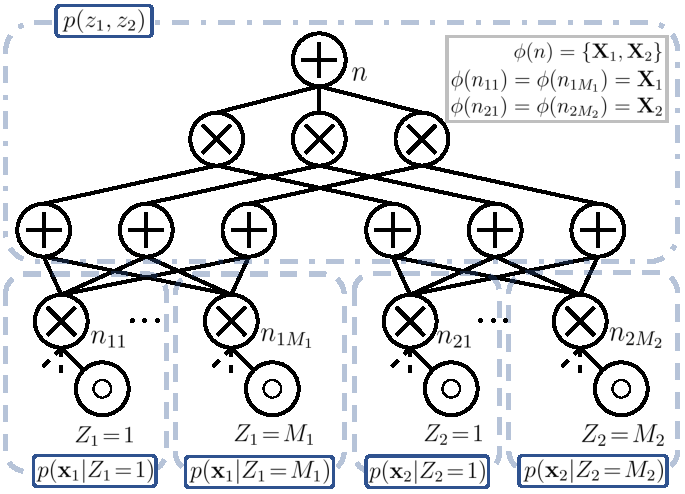
\includegraphics[width=0.46\columnwidth]{figures/fig-pc-decomp.pdf}
    \vspace{-2.0em}
    \caption{Distribution decomposition of an example PC with materialized LVs $Z_1, Z_2$.}
    \label{fig:pc-decomp}
    \vspace{-3.0em}
\end{wrapfigure}


\begin{lem}
\label{lem:independence}
For a PC $\p(\X)$, denote $\W$ as the scope of some units in $\p$. Assume the variable scope of every PC unit is either a subset of $\W$ or disjoint with $\W$. Let $Z$ be the LV corresponds to $\W$ created by \cref{alg:lv}. Then variables $\W$ are conditional independent of $\X \backslash \W$ given $Z$. 
% \guy{see earlier comment, I think this is only true for a carefully chosen order on the edges/latent variables states}
\end{lem}

Proof of the above lemma is provided in \cref{appx:proof1}. Take \cref{fig:add-lvs} as an example. Define the scope of $\{n_i\}_{i=1}^{3}$ and $\{c_i\}_{i=1}^{4}$ as $\W$ and the corresponding LV as $Z$; denote the scope of the full PC as $\X$. \cref{lem:independence} implies that variables $\W$ and $\X \backslash \W$ are conditional independent given $Z$. 

We consider a simple yet effective strategy for materializing LVs: the set of observed variables $\X$ is partitioned into $k$ disjoint subsets $\{\X_i\}_{i=1}^{k}$; then for each $\X_i$, we use \cref{alg:lv} to construct a corresponding LV, termed $Z_i$. As a direct corollary of \cref{lem:independence}, the joint probability over $\X$ and $\Z$ can be decomposed as follows:
% the product of a latent distribution $\p(\Z)$ and multiple latent-conditioned distributions $\{\p(\X_i \given Z_i \!=\! j) : i \!\in\! [k], j \!\in\! [M_i]\}$, where $M_i$ is defined as the number of categories in $Z_i$: 
$\p(\x, \z) \!=\! \p(\z) {\prod}_{i=1}^{k} \p(\x_i \given z_i)$. 

The key to speed up LVD is the observation that the MLE lower bound objective (Eq.~\ref{eq:mle-lowerbound}) can be factored into independent components following the decomposition of $\p(\x, \z)$:
    \begin{align}
        \LL(\p, \data_{\mathrm{aug}}) := \sum_{l=1}^{N} \log \p(\x^{(l)}, \z^{(l)}) = \sum_{l=1}^{N} \sum_{i=1}^{k} \log \p(\x^{(l)}_{i} \given z^{(l)}_{i}) + \sum_{l=1}^{N} \log \p(\z^{(l)}), \label{eq:ll-decomp}
    \end{align}
\noindent where $\data_{\mathrm{aug}} := \{(\x^{(l)}, \z^{(l)})\}_{l=1}^{N}$ is the training set augmented with LV assignments. According to \cref{eq:ll-decomp}, optimize $\LL(\p, \data_{\mathrm{aug}})$ is equivalent to performing MLE on the factorized distributions separately. Specifically, we decompose the optimization process into the following independent steps: (i) for each cluster $i$ and category $j$, optimizing PC parameters \wrt the distribution $\p(\X_i \given Z_i \!=\! j)$ using the subset of training samples whose LV $z_i$ is assigned to category $j$, and (ii) optimizing the sub-PC corresponds to $\p(\z)$ using the set of all LV assignments. Consider the example PC shown in \cref{fig:pc-decomp}. The subset of PC surrounded by every blue box encodes the distribution labeled on its edge. To maximize $\LL(\p, \data_{\mathrm{aug}})$, we can separately train the sub-PCs correspond to the decomposed distributions, respectively. Compared to feeding training samples to the whole PC, the above procedure trains every latent-conditioned distribution $\p(\X_i \given Z_i \!=\! j)$ using only samples that have the corresponding LV assignment (\ie $z_i \!=\! j$), which significantly reduces computation cost.

% \begin{cor}
% \label{cor:pc-decomposition}
% For a PC $\p$ defined on $\X \!:=\! \{\X_i\}_{i=1}^{k}$, define $Z_i$ ($\forall i \!\in\! [k]$) as the LV corresponds to $\X_i$ (materialized by \cref{alg:lv}) and the number of categories in $Z_i$ as $M_i$. $\p$ can be decomposed following the distributions in \cref{eq:pc-lv-decomp}. Moreover, we have \newline
% \textbf{(i)} $\forall i \!\in\! [k], j \!\in\! [M_i]$, the parent of input unit $Z_i \!=\! j$, denoted $n_{ij}$, encodes distribution $\p(\X_i \given Z_i \!=\! j)$; \newline
% \textbf{(ii)} by replacing every $n_{ij}$ with an input unit $Z_i \!=\! j$ (corresponds to the distribution that assigns probability $1$ if $Z_i \!=\! j$ and $0$ otherwise), the resultant PC encodes distribution $\p(\z)$.
% \guy{I don't understand this corollary. Very technical.}
% \end{cor}

% Proof is provided in \cref{appx:proof2}. \cref{fig:pc-decomp} illustrates a PC defined on $\X \!:=\! \{\X_1, \X_2\}$, and with materialized LVs $Z_1$, $Z_2$ correspond to $\X_1$, $\X_2$, respectively. The subset of PC surrounded by every blue box encodes the distribution labeled on its edge. For example, the parent of input unit $Z_1 \!=\! 1$ encodes distribution $\p(\X_1 \given Z_1 \!=\! 1)$, and by replacing PC units $\{n_{ij} : i \!\in\! [k], j \!\in\! [M_i]\}$ with the corresponding input unit specified in \cref{cor:pc-decomposition}, the resultant PC models $\p(Z_1, Z_2)$. Plug in the definition of $\p(\x, \z)$ into the MLE lower bound (Eq.~\ref{eq:mle-lowerbound}), we have 

Recall from \cref{sec:lv-distillation} that in the LVD pipeline, after training the PC parameters by maximizing $\LL (\p, \data_{\mathrm{aug}})$, we still need to finetune the model on the original dataset $\data$. However, this finetuning step often suffers from slow convergence speed, which significantly slows down the learning process. To mitigate this problem, we add an additional \emph{latent distribution training} step where we only finetune parameters correspond to $\p(\Z)$. In this way, we only need to propagate training samples through the sub-PCs correspond to the latent-conditioned distributions once. After this step converges, we move on to finetune the whole model, which then takes much fewer epochs to converge.

% ==========

% As elaborated in \cref{sec:intro}, the main problem of existing EM-based optimizers for PCs is that their E-step is prone to sub-optimal inferred LV assignments. As hinted by \cref{sec:hmm}, supervision of the LVs can be obtained from the less tractable but more expressive generative models such as BERT \citep{devlin2019bert} and Vision Transformers (ViTs) \citep{dosovitskiy2020image}. Such supervision significantly ease the complexity of the optimization tasks given to PC optimizers. For instance, while learning the mixture model in \cref{fig:add-lvs}(a) with the PC defined in \cref{fig:add-lvs}(b) may subject to local optimas, closed-form parameter estimation can be achieved if we obtain $Z$ assignments for all samples from an oracle and use them to learn the equivalent PC in \cref{fig:add-lvs}(c).

% There are three key factors that determine the effectiveness of LV distillation --- (i) what LVs should be chosen for distillation, (ii) how to extract assignments of the selected LVs from expressive generative models, and (iii) how to leverage these assignments to improve PC optimizers. In this section, we assume LVs are chosen wisely and their assignments are obtained from expressive generative models, and focus on demonstrating how the auxiliary information provided by the extracted LVs can be used to improve PC optimizers. Questions (i) and (ii) are left to \cref{sec:extracting-lvs}.

% Before delving into details of the learning algorithm, we take a step back and ask: what properties do we want the materialized LVs to have? While there is no definite answer, we aim to use LVs that concisely and sufficiently represent subsets of the observed variables. Specifically, given observed variables $\X$, we divide them into a set of $k$ mutually exclusive and exhausive variables $\{\X_i\}_{i=1}^{k}$, and assign every $\X_i$ a corresponding LV $Z_i$. Formally, we assume $\p(\X)$ has the following form:
%     \begin{align}
%         \p(\x) = \sum_{\z \in \val(\Z)} \p(\z) \prod_{i=1}^{k} \p(\x_i \given z_i), \quad \text{where~} \forall i,j \in [k] \, (i \neq j), \X_i \!\cap\! \X_j \!=\! \emptyset \text{~and~} \bigcup_{i=1}^{k} \X_i \!=\! \X. 
%     \end{align}
% Another advantage of this LV selection strategy is that it gives every LV clear semantics --- $Z_i$ is an abstract representation of $\X_i$. In the following sections, we first illustrate how to materialize LVs that subject to \cref{eq:pc-lv-decomp} given a PC (Sec.~\ref{sec:pc-lvs}). We then describe the proposed PC parameter learning algorithm that leverages extracted LV assignments (Sec.~\ref{sec:warmup}).

% Now that we have materialized a set of LVs that satisfy \cref{eq:pc-lv-decomp} in a PC, the following step is to optimize the PC with the augmented dataset $\data_{\mathrm{aug}} \!:=\! \{(\x^{(i)}, \z^{(i)})\}_{i=1}^{N}$, where $\z^{(i)}$ is the LV assignment corresponds to $\x^{(i)} \!\in\! \data$ obtained from the generative model. This acquisition process of $\z^{(i)}$ will be detailed in \cref{sec:extracting-lvs}. A straightforward idea is to first maximize the loglikelihood over $(\X, \Z)$: $\LL(\p, \data_{\mathrm{aug}}) := \sum_{i=1}^{N} \log \p(\x^{(i)}, \z^{(i)})$; and then marginalize out $\Z$ and finetune the model by maximizing $\LL(\p, \data) := \sum_{i=1}^{N} \log \p(\x^{(i)})$. However, as we will proceed to show, $\LL(\p, \data_{\mathrm{aug}})$ is not a good surrogate objective for $\LL(\p, \data)$, and the above approach could lead to suboptimal performance.

% As demonstrated in \cref{sec:pc-lvs}, after materializing LVs $\Z$, the PC distribution can be decomposed following \cref{eq:pc-lv-decomp}. In the following corollary, we further show that each of the decomposed distributions is encoded by a subset of PC units, which leads to simple yet effective learning algorithms.

% Since the PCs correspond to distributions $\{\p(\x_i \given Z_i \!=\! j)\}_{i,j}$ and $\p(\z)$ are disjoint (\cref{cor:pc-decomposition}),\footnote{Note that $\forall i \!\in\! [k]$, sub-PCs $\{\p(\x_i \given X_i \!=\! j)\}$ could have shared components. In this case, we need to optimize the distributions with shared PC units jointly, \ie learning the parameters of these sub-PCs by simultaneously maximizing the sum of the corresponding loglikelihood objectives.} maximizing $\LL(\p, \data_{\mathrm{aug}})$ is equivalent to 

% While the objective for $\{\p(\x_i \given Z_i = j)\}_{i,j}$ are desired since they leverage the external guidance from $\Z$, optimizing $\p(\z)$ solely using $\data_{\Z}$ is suboptimal since it does not account for the learning progress of $\{\p(\x_i \given Z_i \!=\! j)\}_{i,j}$. A better objective should directly optimize $\p(\z)$ to maximize $\LL(\p, \data)$. Recall that the subset of PC corresponds to the latent-conditioned distributions $\{\p(\x_i \given Z_i \!=\! j)\}_{i,j}$ can be trained independently with $\{\data_{ij}\}_{i,j}$, respectively. This allows us to first train the latent-conditioned distributions and then treat them as constants when training $\p(\z)$ to maximize $\LL(\p, \data)$. According to \cref{cor:pc-decomposition}, computing $\p(\x) \!=\! \sum_{\z \in \val(\Z)} \p(\z) \prod_{i=1}^{k} \p(\x_i \given z_i)$ is equivalent to performing a feedforward pass over the PC given input $\x$.\footnote{The feedforward pass computes the output probability of every PC unit following \cref{eq:pc-def}, children before parents. Note that variables $\Z$ are marginalized out, which is implemented by setting the output of all input units correspond to variables in $\Z$ to $1$.} Therefore, optimize $\p(\z)$ \wrt $\LL(\p, \data)$ is equivalent to optimize the whole PC $\p(\x)$ while fixing the parameters correspond to PC units $\{\p(\x_i \given Z_i \!=\! j)\}_{i,j}$. In summary, we first optimize sub-PCs correspond to $\{\p(\x_i \given Z_i \!=\! j)\}_{i,j}$ using $\{\data_{ij}\}_{i,j}$, respectively. We then fix these PC units and only optimize the parameters of PC units correspond to $\p(\z)$ with the original dataset $\data$. We use stochastic mini-batch EM for both steps, which is detailed in \cref{appx:em}.

% \section{Extracting LVs from Expressive Generative Models}
\section{Extracting Latent Variables for Image Modeling}
\label{sec:extracting-lvs}

This section discusses how to induce assignments to LVs using expressive generative models. While the answer is specific to individual data types, we proposes preliminary answers of the question in the context of image data. We highlight that there are many possible LV selection strategies and target generative model; the following method is only an example that shows the effectiveness of LVD.

Motivated by recent advances of image-based deep generative models \citep{dosovitskiy2020image,liu2021swin}, we model images by two levels of hierarchy --- the low-level models independently encode distribution of every image patch, and the top-level model represents the correlation between different patches. Formally, we define $\X_i$ as the variables in the $i$th $M \times M$ patch of an $H \times W$ image (w.l.o.g. assume $H$ and $W$ are both divisible by $M$). Therefore, the image $\X$ is divided into $k = H \cdot W / M^2$ subsets $\{\X_i\}_{i=1}^{k}$. Every $Z_i$ is defined as the LV corresponds to patch $\X_i$.

\begin{figure}
    \centering
    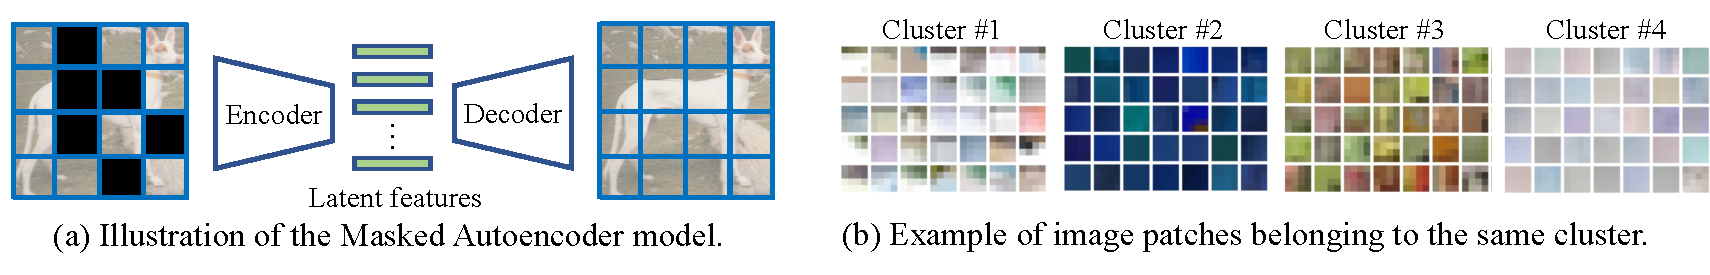
\includegraphics[width=\columnwidth]{figures/fig-mae.pdf}
    \vspace{-2.0em}
    \caption{Extracting LVs for image data. The MAE model (a) is used to extract categorical LVs $\{Z_i\}_{i=1}^{k}$ that correspond to image patches $\{\X_i\}_{i=1}^{k}$, respectively. (b) provides example patches from the training set that belong to four randomly chosen clusters of the LV $Z_1$.}
    \label{fig:mae}
\end{figure}

Recall that our goal is to obtain the assignment of $\{Z_i\}_{i=1}^{k}$, each as a concise representation of $\{\X_i\}_{i=1}^{k}$, respectively. Despite various possible model choices, we choose to use Masked Autoencoders (MAEs) \citep{he2022masked} as they produce good features for image patches. Specifically, as shown in \cref{fig:mae}(a), MAE consists of an encoder and a decoder. During training, a randomly selected subset of patches are fed to the encoder to generate a latent representation for every patch. The features are then fed to the decoder to reconstruct the full image. The simplest way to compute latent features for every patch is to feed them into the encoder independently, and extract the corresponding features. However, we find that it is beneficial to also input other patches as context. Specifically, we first compute the latent features without context. We then compute the correlation between features of all pair of patches and construct the Maximum Spanning Tree (MST) using the pairwise correlations. Finally, to compute the feature of each patch $\X_i$, we additionally input patches correspond to its ancestors in the MST. Further details are given in \cref{appx:mae}.

As shown in \cref{sec:lv-distillation}, LVs $\{Z_i\}_{i=1}^{k}$ are required to be categorical. To achieve this, we run the K-means algorithm on the latent features (of all training examples) and use the resultant cluster indices as the LV assignments. \cref{fig:mae}(b) shows some example image patches $\x_1$ belonging to four latent clusters (\ie $Z_1 = 1, \dots, 4$). Clearly, the LVs capture semantics of different image patches.

To illustrate the effectiveness of LVD, we make minimum structural changes compared to Hidden Chow-Liu Trees (HCLTs) \citep{liu2021tractable}, a competitive PC structure. Specifically, we use the HCLT structure for all sub-PCs $\{\p(\x_i \given Z_i \!=\! j)\}_{i,j}$ and $\p(\z)$. This allows us to materialize patch-based LVs while keeping the model architecture similar to HCLTs.

\section{Experiments}
\label{sec:exp}

In this section, we evaluate the proposed latent variable distillation (LVD) technique on three natural image benchmarks, \ie CIFAR \citep{krizhevsky2009learning} and two versions of down-sampled ImageNet (ImageNet32 and ImageNet64) \citep{deng2009imagenet}. On all benchmarks, we demonstrate the effectiveness of LVD from two perspectives. First, compared to PCs trained by existing EM-based optimizers, the proposed technique offers a significant performance gain especially on large PCs. Second, PCs trained by LVD achieve competitive performance against some of the less tractable deep generative models, including variational autoencoders and flow-based models.

\begin{table*}[t]
\caption{Density estimation performance of Tractable Probabilistic Models (TPMs) and Deep Generative Models (DGMs) on three natural image datasets. Reported numbers are test set bit-per-dimension (bpd). Bold indicates best bpd (smaller is better) among all four TPMs.}
\label{tab:img-main-results}
\centering
\scalebox{1.0}{
\begin{tabular}{lccccccc}
    \toprule
    \multirow{2}{*}[-0.2em]{Dataset} & \multicolumn{4}{c}{TPMs} & \multicolumn{3}{c}{DGMs} \\
    \cmidrule(lr){2-5}
    \cmidrule(lr){6-8}
    ~ & LVD (ours) & HCLT & EiNet & RAT-SPN & Glow & RealNVP & BIVA \\
    \midrule
    ImageNet32 & \textbf{4.38} & 4.82 & 5.63 & 6.90 & 4.09 & 4.28 & 3.96 \\
    ImageNet64 & \textbf{4.12} & 4.67 & 5.69 & 6.82 & 3.81 & 3.98 & - \\
    CIFAR & \textbf{4.37} & 4.61 & 5.81 & 6.95 & 3.35 & 3.49 & 3.08 \\
    \bottomrule
\end{tabular}
}
\vspace{-1.0em}
\end{table*}

\boldparagraph{Baselines} We compare the proposed method against three TPM baselines: Hidden Chow-Liu Tree (HCLT) \citep{liu2021tractable}, Einsum Network (EiNet) \citep{peharz2020einsum}, and Random Sum-Product Network (RAT-SPN) \citep{peharz2020random}. Though not exhausive, this baseline suite embodies many of the recent advancement in tractable probabilistic modeling, and can be deemed as the existing SoTA. To evaluate the performance gap with less tractable deep generative models, we additionally compare LVD with the following flow-based and VAE models: Glow \citep{kingma2018glow}, RealNVP \citep{dinh2016density}, and BIVA \citep{maaloe2019biva}.

To facilitate a fair comparison with the chosen TPM baselines, we implement both HCLT and RAT-SPN using the Julia package Juice.jl \citep{dang2021juice} and tune hyperparameters such as batch size, learning rate and its schedule. We use the original PyTorch implementation of EiNet and similarly tune their hyperparameters. For all TPMs, we train various models with number of parameters ranging from $\sim$1M to $\sim$100M, and report the number of the model with the best performance. For deep generative model baselines, we adopt the numbers reported in the respective original papers. Please refer to \cref{sec:exp-details} for more details of the experiment setup.

\begin{figure}
    \centering
    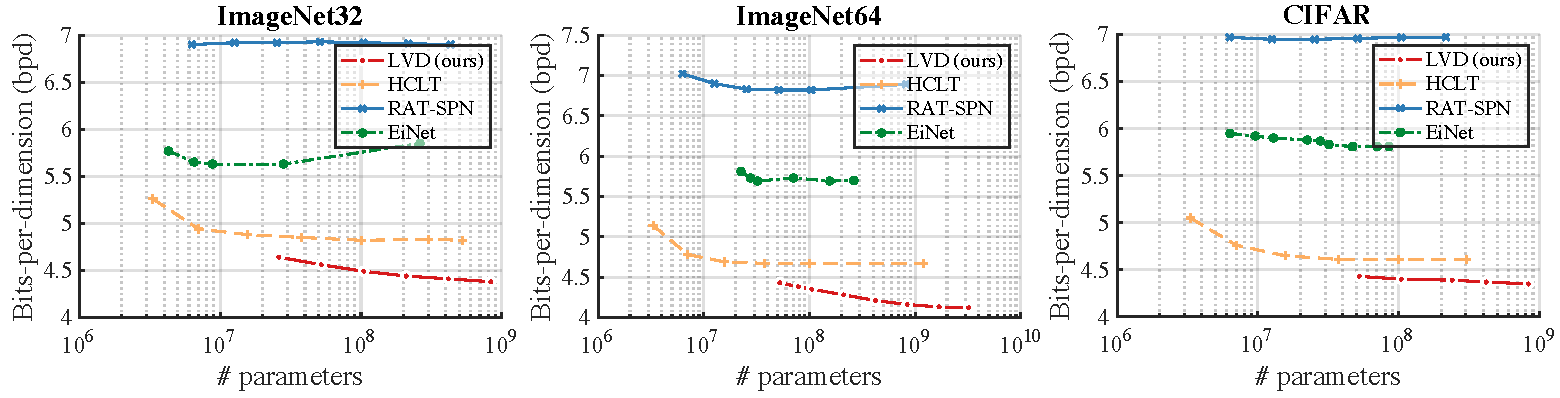
\includegraphics[width=\columnwidth]{figures/fig-img-results.pdf}
    \vspace{-1.8em}
    \caption{Generative modeling performance of four TPMs on three natural image datasets. For each method, we report the test set bits-per-dimension (y-axis) in terms of the number of parameters (x-axis) for different numbers of latent states.}
    \label{fig:img-results}
\end{figure}

\boldparagraph{Empirical Insights} We first compare the performance of the four TPM approaches. As shown in \cref{fig:overview-res}, for all three benchmarks, PCs trained by LVD are consistently better than the competitors by a large margin. In particular, on ImageNet32, a $\sim$25M PC trained by LVD is better than a HCLT with $\sim$400M parameters. Next, looking at individual curves, we observe that with LVD, the test set bpd keeps decreasing as the model size increases. This indicates that LVD is able to take advantage of the extra capacity offered by large PCs. In contrast, PCs trained by EM immediately suffer from a performance bottleneck as the model size increases. Additionally, the efficient LVD learning pipeline described in \cref{sec:efficient-pc-learning} allows us to train PCs with 500M parameters in 10 hours with a single NVIDIA A5000 GPU, while existing optimizers need over 1 day to train baseline PCs with similar sizes.

We move on to compare the performance of LVD with the three adopted DGM baselines. As shown in \cref{tab:img-main-results}, although the performance gap is relatively large on CIFAR, the performance of LVD is highly competitive on ImageNet32 and ImageNet64, with bpd gap ranging from $\sim\!0.1$ to $\sim\!0.3$. We hypothesize that the relatively large performance gap on CIFAR is caused by insufficient training samples. Specifically, for the PC structures specified in \cref{sec:extracting-lvs}, the sub-PCs correspond to the latent-conditioned distributions $\{\p(\x_i \given Z_i \!=\! j)\}_{i,j}$ are constructed independently, and thus every training sample $\x_i$ can only be used to train its corresponding latent-conditioned distribution, making the model extremely data-hungry. However, we note that this is not an inherent problem of LVD. For example, by performing parameter tying of sub-PCs correspond to different image patches, we can significantly improve sample complexity of the model. This is left to future work.

\vspace{-0.4em}
\section{Related Works}
\vspace{-0.4em}

There has been various recent endeavors to improve the performance of PCs on modeling complex and high-dimensional datasets. An extensively-explored direction is to construct or learn the structure of PCs that is tailored to the target dataset. For example, \citet{gens2013learning,dang2022sparse} seek to progressively improve the PC structure during the optimization process. Many other work aim to construct good PC structures given the dataset in one shot, and then move on to parameter optimization \citep{rahman2014cutset,adel2015learning}. Model agnostic PC structures such as RAT-SPN \citep{peharz2020random} and extremely randomized PCs (XPCs) \citep{di2021random} are also shown effective in various density estimation benchmarks. There are also papers that focus exclusively on scaling up a particular TPM. For example, scaling HMM \citep{chiu-rush-2020-scaling} uses techniques such as learning blocked emission probabilities to boost the performance of HMMs.

Another line of work seek to scale up PCs by learning hybrid models with neural networks (NNs). Specifically, \citet{shao2022conditional} leverages the expressive power of NNs to learn expressive yet tractable conditional distributions; HyperSPN \citep{shih2021hyperspns} uses NN to regularize PC parameters, which prevents large PCs from overfitting. Such hybrid models are able to leverage the expressiveness of NNs at the cost of losing tractability on certain queries.

% HyperSPN~\citep{shih2021hyperspns}.
% Scaling HMM~\citep{chiu-rush-2020-scaling}.
% extremely randomized PCs (XPCs)~\citep{di2021random}.
% PC/SPN structure learning~\citep{gens2013learning,dang2022sparse,rahman2014cutset,adel2015learning}.
% SPN parameter learning~\citep{zhao2016unified}.

\vspace{-0.4em}
\section{Conclusion}
\vspace{-0.4em}

Scaling probabilistic circuits to large and high-dimensional real-world datasets has been a key challenge: as the number of parameters increases, their performance gain diminishes immediately. In this paper, we propose to tackle this problem by latent variable distillation: a general framework for training probabilistic circuit that provides extra supervision over their latent spaces by distilling information from existing deep generative models. The proposed framework significantly boosts the performance of large probabilistic circuits on challenging benchmarks for both image and language modeling. In particular, with latent variable distillation, a image-patch-structured probabilistic circuit achieves competitive performance against flow-based models and variational autoencoders. Despite its empirical success on scaling up probabilistic circuits, at high-level, latent variable distillation also implies a new way to organically combine probabilistic circuits and neural models, opening up new avenues for tractable generative modeling.

\paragraph{Reproducibility statement} To facilitate reproducibility, we provide detailed description of the models and training details in both the main text and the appendix. Specifically, the last paragraph in \cref{sec:extracting-lvs} elaborates the PC structure used for image modeling tasks; training details of both the proposed method and the baselines are provided in \cref{sec:exp,sec:exp-details}. For baselines, we always use the official GitHub implementation if possible. For our method, we provide detailed explanation of all hyperparameters used in the experiment (\cref{sec:exp-details}).

\bibliography{iclr2023_conference}
\bibliographystyle{iclr2023_conference}

\newpage
\appendix

\section{Proofs}

In this section, we provide detailed proofs of \cref{lem:independence}.

\subsection{Proof of Lemma \ref{lem:independence}}
\label{appx:proof1}

\begin{proof}
Define $\Y \!:=\! \X \backslash \W$. To prove that variables $\W$ is conditional independent with $\Y$ given $Z$, it is sufficient to show that $\forall \w \!\in\! \val(\W), z \!\in\! \val(Z), \y \!\in\! \val(\Y)$, we have $\p(\w \given z) \!=\! \p(\w \given z, \y)$.

Define $S_{\p,\W}^{\mathrm{sum}}$ and $S_{\p,\W}^{\mathrm{prod}}$ as the set of sum and product units with scope $\W$, respectively. $\forall n \!\in\! S_{\p,\W}^{\mathrm{sum}}$, since the scope of $n$ does not contain variables $\Y$, we can immediately conclude that $\p_{n} (\w \given z) \!=\! \p(\w \given z, \y)$. In order to show that this equation also holds for the root PC unit, we only need to show that for each PC unit $n$ in $\p$, if all its children (whose scope contains $\W$) satisfy this equation, then $n$ also does. The reason is that the root unit $n_r$ of $\p$ must be an ancestor unit of every unit in $S_{\p,\W}^{\mathrm{sum}}$.

We start with the case that $n$ is a product unit. Since the PC is assumed to be decomposable, only one child, denoted $m$, satisfies $\W \subseteq \scope(m)$. Therefore, the distribution of $n$ can be written as
    \begin{align*}
        \p_{n} (\x) = \p_{m} (\x) \cdot \prod_{c \in \ch(n), c \neq m} \p_{c} (\x) \overset{(a)}{=} \p_{m} (\x) \cdot \prod_{c \in \ch(n), c \neq m} \p_{c} (\y),
    \end{align*}
\noindent where $(a)$ holds because $\forall c \!\in\! \ch(n), c \!\neq\! m$, we have $\phi(c) \cap \W = \emptyset$. Therefore, we have $\p_{n} (\w \given z) = \p_{m} (\w \given z)$ and $\p_{n} (\w \given z, \y) = \p_{m} (\w \given z, \y)$. Taking the two equations together and use the assumption from the induction step: $\p_{m} (\w \given z) \!=\! \p_{m} (\w \given z, \y)$, we conclude that $\p_{n} (\w \given z) \!=\! \p_{n} (\w \given z, \y)$.

Define $n_z$ as the product unit in $S_{\p,\W}^{\mathrm{prod}}$ that is augmented with input unit $Z = z$ by \cref{alg:lv}. Before proving the main result, we highlight that $\forall n$ whose scope contains $\W$, $\p_{n}(\x)$ can be written as $\p_{n_{z}}(\w) \cdot g_{n}(\y)$, where $g_{n}(\y)$ is independent with $\w$. This is because $\forall m \in S_{\p,\W}^{\mathrm{prod}}$ and $m \neq n_z$, $\p_{m}(\w,z) = 0 (\forall \w \in \val(\W))$.

Next, assume $n$ is a sum unit whose scope contains $\W$. Using the above result, we know that every child $c$ of $n$ satisfies the following: $\p_{c} (\x) = \p_{n_{z}}(\w) \cdot g_{c}(\y)$. Thus, we have
    \begin{align*}
        \p_{n} (\x) = \sum_{c \in \ch(n)} \theta_{c \given n} \cdot \p_{n_{z}}(\w) \cdot g_{c}(\y) = \p_{n_{z}}(\w) \cdot \Big ( \sum_{c \in \ch(n)} \theta_{c \given n} \cdot g_{c}(\y) \Big ).
    \end{align*}
Since $\p_{n_z} (\w \given z) \!=\! \p_{n_z} (\w \given z, \y)$, we have $\p_{n} (\w \given z) \!=\! \p_{n} (\w \given z, \y)$.

Taking the above two inductive cases (\ie for sum and product units, respectively), we can conclude that for the root unit $n_r$, $\p_{n_r} (\w \given z) \!=\! \p_{n_r} (\w \given z, \y)$.
\end{proof}

% \subsection{Proof of Corollary \ref{cor:pc-decomposition}}
% \label{appx:proof2}

% \begin{proof}
% Recall from \cref{appx:proof1} that for every PC unit $n$ whose scope contains $\W$, we have
%     \begin{align}
%         \p_{n} (\x) = \p_{n_z} (\w) \cdot g_{n} (\y), \label{eq:proof2-1}
%     \end{align}
% \noindent where $Z$ is the LV corresponds to $\W$ (materialized by \cref{alg:lv}), and $n_z$ is the parent product unit of the input unit $Z \!=\! z$.

% Now assume $\X \!:=\! \{\X_i\}_{i=1}^{k}$ and define $Z_i$ as the LV of $\X_i$ materialized by \cref{alg:lv}. Denote $n_r$ as the root unit of the PC. Following the above result (\cref{eq:proof2-1}), we have that $\forall i \!\in\! [k], j \!\in\! [M_i]$,
%     \begin{align*}
%         \p_{n_r} (\x) = \p_{n_{ij}} (\x_{i}) \cdot g_{n_r,i}(\x \backslash \x_{i}, \z),
%     \end{align*}
% \noindent where $g_{n_r,i}(\x \backslash \x_{i}, \z)$ is independent with $\x_i$. Thus, for every $\x_i \!\in\! \val(\X_i, z_i)$, we have $\p_{n_r} (\x_i, z_i) = \p_{n_{ij}} (\x_i) \cdot g_{n_r,i}(z_i)$ and $\p_{n_r} (z_i) = 1 \cdot g_{n_r,i}(z_i)$. Therefore, we conclude that $\p(\x_i \given Z_i \!=\! j) = \p_{n_{ij}} (\x_i)$, which is the first conclusion in \cref{cor:pc-decomposition}.

% To proof the second conclusion, we observe that when computing $\p_{n_r}(\z)$ following a feedforward pass, we have $\p_{n_{ij}} (\z) = \mathbbm{1}[z_i \!=\! j]$, where $\mathbbm{1}[\cdot]$ is the indicator function. This is because the scope of $n_{ij}$ is $\X_i \cup Z_i$ and all $\X_i$ variables are marginalized out. Therefore, by replacing every $n_{ij}$ with an input unit $Z_i \!=\! j$, the resultant PC encodes distribution $\p(\Z)$.
% \end{proof}

\section{Details for Latent Variable Distillation}

This section provides additional details for latent variable distillation~(LVD), including description of the adopted EM algorithm and details of the LV extraction step.

\subsection{Parameter Estimation}
\label{appx:em}

We adopt a stochastic mini-batch version of the Expectation-Maximization algorithm. Specifically, a mini-batch of samples are drown from the dataset, and the EM algorithm for PCs \citep{choi2021group,dang2021juice} is used to compute a set of new parameters $\params^{\mathrm{new}}$, which is updated with a learning rate $\alpha$: $\params_{t+1} \leftarrow \alpha \!\cdot\! \params^{\mathrm{new}} + (1-\alpha) \!\cdot\! \params_{t}$.

\subsection{Details of the MAE-based LV Extraction Step}
\label{appx:mae}

We use the official code (\url{https://github.com/facebookresearch/mae}) to train MAE models on the adopted datasets (\ie CIFAR, ImageNet32, and ImageNet64). At each training step, the percentage of masked patches is chosen uniformly from 10\% to 90\%. After training, the LV extraction step follows the description in \cref{sec:extracting-lvs}.

\section{Experiment Details}
\label{sec:exp-details}

In this section, we describe experiment details of all four TPMs adopted in \cref{sec:hmm} and \cref{sec:exp}.

\boldparagraph{Hardware specification} All experiments are run on servers/workstations with the following configuration:

$\bullet$ 32 CPUs, 128G Mem, 4 $\times$ NVIDIA A5000 GPU;

$\bullet$ 32 CPUs, 64G Mem, 1 $\times$ NVIDIA GeForce RTX 3090 GPU;

$\bullet$ 64 CPUs, 128G Mem, 3 $\times$ NVIDIA A100 GPU.

\boldparagraph{HMM}
The HMM models are trained with varying hidden states $h$ = 128, 256, 512, 750, 1024 and 1250, with and without LVD. All HMM models are trained with mini-batch EM (\cref{appx:em}) for two phases: in phase 1, the model is trained with learning rate $0.1$ for 20 epochs; in phase 2, the model is trained with learning rate $0.01$ for 5 epochs. Note that for HMM models with hidden states $\geq$ 750, we train for 30 epochs in phase 1. The number of epochs are selected such that all model converges before training stops.

\boldparagraph{LVD} For every subset $\X_i$, the number of hidden categories, \ie $\{M_i\}_{i=1}^{k}$ are set to values in $\{8, 16, 32, 64, 128, 256\}$. For the latent-conditioned distribution $\{\p(\X_i \given Z_i \!=\! j)\}_{i,j}$, we adopt HCLTs with hidden size 16, and for the latent distribution $\p(\Z)$, a HCLT with hidden size $M_i$ is adopted. When optimizing the model with the MLE lower bound, we adopt mini-batch EM (\cref{appx:em}) with learning rate annealed linearly from $0.1$ to $0.01$. In the latent distribution training step (Sec.~\cref{sec:efficient-pc-learning}), we anneal learning rate from $0.1$ to $0.001$.

\boldparagraph{HCLT} We use the publicly available implementation of HCLT at \url{https://github.com/Juice-jl/ProbabilisticCircuits.jl/blob/master/src/structures/hclts.jl}. The hidden size is chosen from $\{16, 32, 64, 128, 256, 512, 1024\}$. We anneal the EM learning rate from $0.1$ to $0.01$ and train for 100 epochs, and then anneal the learning rate from $0.01$ to $0.001$ and train for another 100 epochs.

\boldparagraph{RAT-SPN} We adopt the publicly available implementation at \url{https://github.com/Juice-jl/ProbabilisticCircuits.jl/blob/master/src/structures/rat.jl}. \textsf{num\_nodes\_region}, \textsf{num\_features}, and \textsf{num\_nodes\_leaf} are set to the same value, which is chosen from $\{16, 32, 64, 128, 256, 512, 1024\}$. Learning rate schedule is same with HCLTs.

\boldparagraph{EiNet} We use the official implementation on GitHub: \url{https://github.com/cambridge-mlg/EinsumNetworks}. We use the PD structure provided in the codebase. We select hyperparameter \textsf{delta} from $\{4, 6, 8\}$ and select \textsf{num\_sums} from $\{16, 32, 64, 128, 256\}$. Learning rate is set to $0.001$.

\end{document}
